\documentclass[../../dis.tex]{subfiles}
\begin{document}
\chapter{L3 - Storage, Files, and Indexing}\label{chap:l3}
\newpage
\section*{Extra: SQL in the era of AI}
Large language models (LLMs) make one question unavoidable: will natural language (NL) replace SQL? Will people soon query databases in plain English?

\begin{concept}{NL2SQL systems}
AI systems that turn natural language into SQL queries. Examples include Palimpzest and Lotus. They act as a \emph{front-end}: they help users ask, draft, and explain queries, but they do not replace the database itself.
\end{concept}

Databases and LLMs play different roles:
\begin{dashlist}
    \item \textbf{DBMS (Back-end)}: Stores data, enforces constraints, manages transactions, controls access, and executes queries efficiently.
    \item \textbf{LLM (Front-end)}: Turns prompts into text or code, but gives \textbf{no correctness guarantees}.
\end{dashlist}
\subsection*{Current limitations of NL2SQL}
These tools are useful, but they still need careful checking:
\begin{dashlist}
    \item People still outperform the best current systems (for example, $93\%$ vs. $82\%$ on the BIRD benchmark).
    \item Execution accuracy drops significantly as query difficulty increases.
    \item Common AI errors include wrong joins, wrong aggregation level, missing \texttt{DISTINCT}, and wrong filter order.
\end{dashlist}

\subsection*{Why relational reasoning still matters}
SQL and the relational model give \textbf{precision, composability, and optimization}. Even if natural language becomes the visible interface, the database still runs on these ideas.

If you do not understand SQL and relational reasoning, you cannot:
\begin{dashlist}
    \item \textbf{Verify} the correctness of AI-generated queries.
    \item \textbf{Debug} query failures or logical errors.
    \item \textbf{Predict} and optimize database performance.
\end{dashlist}
\newpage
\section{File and access layer}
At the physical level, a database is a \textbf{file of records}. The DBMS stores these records in operating-system files and supports a small set of access operations.

The main operations at this layer are:
\begin{dashlist}
    \item create and delete files,
    \item insert, delete, and update records,
    \item \textbf{point access}: retrieve one record via its identifier,
    \item \textbf{range access}: retrieve all records satisfying a condition,
    \item \textbf{scan}: read the entire file.
\end{dashlist}

\subsection{File organization and indexing}
This layer answers three questions:
\begin{dashlist}
    \item how records are stored in files,
    \item how indexes speed up access,
    \item how pages are placed on storage.
\end{dashlist}

Metadata about these choices is stored in the \emph{system catalog}.

\begin{concept}{Storage hierarchy}
Database storage has levels:
\begin{dashlist}
    \item a \textbf{file} is a set of \textbf{pages} (blocks),
    \item a \textbf{page} stores multiple \textbf{records},
    \item a \textbf{record} is a sequence of \textbf{fields}.
\end{dashlist}
\end{concept}

\begin{figure}[htp]
\centering
{\begin{tikzpicture}[
    x=1cm,y=1cm,
    scale=1.00,
    transform shape,
    every node/.style={font=\small},
    >=Latex,
    frame/.style={draw=black!60, rounded corners=3pt, line width=0.85pt},
    stage/.style={frame, fill=gray!5, minimum width=2.55cm, minimum height=2.25cm},
    recordstage/.style={stage, minimum width=4.80cm},
    filebox/.style={frame, fill=blue!6, minimum width=1.58cm, minimum height=0.38cm},
    pagebox/.style={frame, fill=cyan!7, minimum width=1.58cm, minimum height=0.30cm},
    recbox/.style={frame, fill=green!10, minimum width=1.58cm, minimum height=0.30cm},
    fieldbox/.style={frame, fill=orange!14, minimum height=0.60cm, inner xsep=4pt},
    flow/.style={->, thick, draw=black!55}
]
    \node[stage] (db) at (0,0) {};
    \node[font=\bfseries] at (0,1.45) {Database};
    \node[filebox] at (0,0.55) {File A};
    \node[filebox] at (0,0.00) {File B};
    \node[filebox] at (0,-0.55) {File C};

    \node[stage] (file) at (3.65,0) {};
    \node[font=\bfseries] at (3.65,1.45) {File};
    \node[pagebox] at (3.65,0.68) {Page 0};
    \node[pagebox] at (3.65,0.20) {Page 1};
    \node[pagebox] at (3.65,-0.28) {Page 2};
    \node[pagebox] at (3.65,-0.76) {Page 3};

    \node[stage] (page) at (7.30,0) {};
    \node[font=\bfseries] at (7.30,1.45) {Page};
    \node[recbox] at (7.30,0.68) {Record 0};
    \node[recbox] at (7.30,0.20) {Record 1};
    \node[recbox] at (7.30,-0.28) {Record 2};
    \node[recbox] at (7.30,-0.76) {Record 3};

    \node[recordstage] (record) at (12,0) {};
    \node[font=\bfseries] at (12,1.45) {Record};
    \node[fieldbox] at (10.5,0) {id};
    \node[fieldbox] at (11.5,0) {name};
    \node[fieldbox] at (12.5,0) {dept};
    \node[fieldbox] at (13.5,0) {gpa};
    \node[font=\scriptsize] at (12,-0.78) {Fields};

    \draw[flow] (db.east) -- (file.west);
    \draw[flow] (file.east) -- (page.west);
    \draw[flow] (page.east) -- (record.west);
\end{tikzpicture}
}\par}
\end{figure}

Physical design means choosing a file organization, managing free space, and adding indexes for fast access.
\newpage
\section{Page and record formats}
Most databases use the N-ary storage model (row store): each page stores many complete tuples, one per slot.

\begin{concept}{Record Identifier (RID)}
A record is usually identified by its page id and slot number, often written $\langle \text{page\_id}, \text{slot\_number} \rangle$. Some systems show a logical identifier instead, but it still maps to a page and a slot.
\end{concept}

A page format must support search, insertion, and deletion efficiently. The first question is whether records are \textbf{fixed-length} or \textbf{variable-length}.

\begin{figure}[htp]
\centering
\begin{minipage}{0.39\textwidth}
Once the DBMS finds the right page, the slot number points to the record inside that page. \textbf{Keeping this identifier stable is one of the main goals of page design.}
\end{minipage}
\hfill
\begin{minipage}{0.56\textwidth}
{\centering\begin{tikzpicture}[
    x=1cm,y=1cm,
    every node/.style={font=\small},
    frame/.style={draw=black!60, rounded corners=3pt, line width=0.85pt},
    slot/.style={frame, fill=blue!7, minimum width=1.15cm, minimum height=0.72cm},
    hit/.style={frame, fill=orange!16, minimum width=1.15cm, minimum height=0.72cm},
    >=Latex
]
    \draw[frame, fill=gray!4] (0,0) rectangle (5.8,3.3);
    \draw[frame, fill=gray!14] (0,2.55) rectangle (5.8,3.3);
    \node[font=\bfseries] at (2.9,2.93) {Page 42};
    \node[font=\scriptsize] at (0.75,2.93) {header};

    \node[slot] at (1.0,1.85) {slot 0};
    \node[slot] at (2.35,1.85) {slot 1};
    \node[slot] at (3.70,1.85) {slot 2};
    \node[hit]  (rid) at (5.05,1.85) {slot 3};
    \node[slot] at (1.0,0.85) {slot 4};
    \node[slot] at (2.35,0.85) {slot 5};
    \node[slot] at (3.70,0.85) {slot 6};
    \node[slot] at (5.05,0.85) {slot 7};

    \node[align=center] (label) at (3.8,-0.45) {$\mathrm{RID}=\langle 42,3\rangle$};
    \draw[->, thick, draw=black!55] (label.north) to[out=110,in=-60] (rid.south);
\end{tikzpicture}
}\par}
\end{minipage}
\end{figure}

\subsection{Fixed-length records}
If all fields have fixed size, for example integers or fixed-size \texttt{char} values, then every record has the same length:
\begin{dashlist}
    \item the schema is fixed and stored in the catalog,
    \item field $i$ starts at a fixed offset,
    \item pages can use very simple slot layouts.
\end{dashlist}

\subsubsection*{Fixed-length page layouts}
\begin{figure}[htp]
\centering
\begin{minipage}{0.48\textwidth}
\centering
\textbf{Packed page}
\par\smallskip

{\begin{tikzpicture}[
    x=1cm,y=1cm,
    every node/.style={font=\small},
    frame/.style={draw=black!60, rounded corners=3pt, line width=0.85pt},
    rec/.style={frame, fill=blue!7, minimum width=1.0cm, minimum height=1.0cm},
    gap/.style={draw=red!70!black, rounded corners=3pt, line width=0.9pt, dashed, minimum width=1.0cm, minimum height=1.0cm},
    >=Latex
]
    \draw[frame, fill=gray!4] (0,0) rectangle (5.9,1.8);
    \node[font=\bfseries] at (2.95,2.15) {Contiguous records};

    \node[rec] at (0.75,0.9) {R0};
    \node[rec] at (1.90,0.9) {R1};
    \node[gap] at (3.05,0.9) {delete};
    \node[rec] at (4.20,0.9) {R3};
    \node[rec] at (5.35,0.9) {R4};

    \draw[->, thick, draw=black!55] (5.35,-0.25) -- (3.55,-0.25);
    \node[font=\scriptsize, align=center] at (4.45,-0.70) {later records shift left};
\end{tikzpicture}
}\par}
\smallskip

\raggedright
Records are stored next to each other, so space usage is very good. The downside is that deleting one record shifts later records and changes their RIDs.
\end{minipage}
\hfill
\begin{minipage}{0.48\textwidth}
\centering
\textbf{Bitmap page}
\par\smallskip

{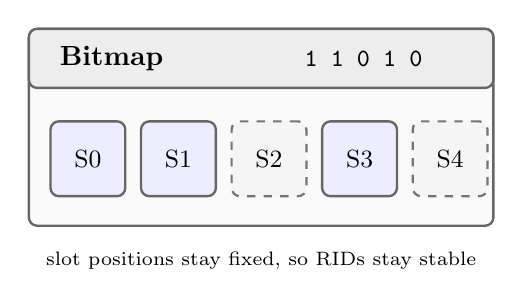
\begin{tikzpicture}[
    x=1cm,y=1cm,
    every node/.style={font=\small},
    frame/.style={draw=black!60, rounded corners=3pt, line width=0.85pt},
    slot/.style={frame, fill=blue!7, minimum width=0.95cm, minimum height=0.95cm},
    empty/.style={draw=black!55, rounded corners=3pt, line width=0.8pt, dashed, fill=gray!8, minimum width=0.95cm, minimum height=0.95cm}
]
    \draw[frame, fill=gray!4] (0,0) rectangle (5.9,2.5);
    \draw[frame, fill=gray!14] (0,1.75) rectangle (5.9,2.5);
    \node[font=\bfseries] at (1.05,2.12) {Bitmap};
    \node[font=\ttfamily\small] at (4.25,2.12) {1 1 0 1 0};

    \node[slot]  at (0.75,0.85) {S0};
    \node[slot]  at (1.90,0.85) {S1};
    \node[empty] at (3.05,0.85) {S2};
    \node[slot]  at (4.20,0.85) {S3};
    \node[empty] at (5.35,0.85) {S4};

    \node[font=\scriptsize, align=center] at (2.95,-0.45) {slot positions stay fixed, so RIDs stay stable};
\end{tikzpicture}
}\par}
\smallskip

\raggedright
A bitmap shows which fixed slots are in use. When a record is deleted, its bit is cleared. The empty slot can be reused later, and record positions stay stable.
\end{minipage}
\end{figure}

\subsection{Variable-length records}
We need variable-length layouts when records contain fields such as \texttt{varchar}, or when one file stores several record types.

A common layout contains:
\begin{dashlist}
    \item fixed-size values at the front,
    \item one $\langle \text{offset}, \text{length} \rangle$ entry per variable field,
    \item the actual variable-length data at the end,
    \item a small null bitmap for missing attributes.
\end{dashlist}

\begin{figure}[htp]
\centering
{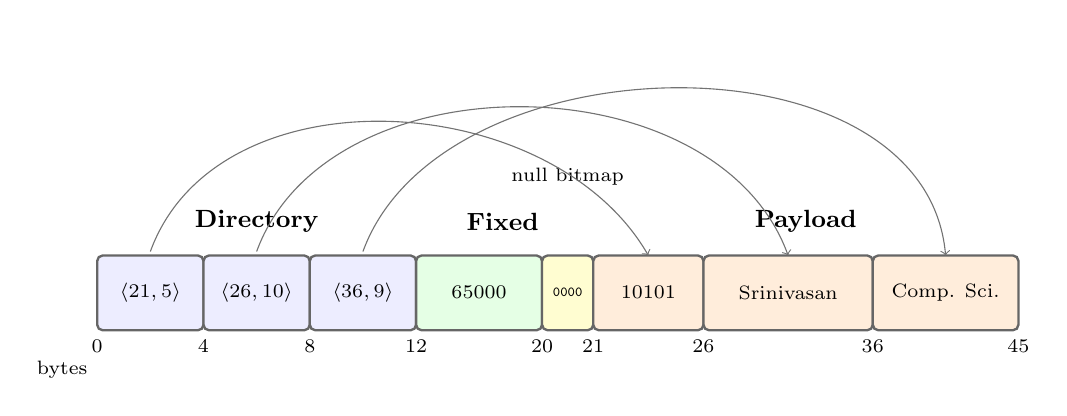
\begin{tikzpicture}[
    x=1cm,y=1cm,
    every node/.style={font=\scriptsize},
    frame/.style={draw=black!60, rounded corners=2pt, line width=0.85pt},
    dir/.style={frame, fill=blue!7},
    fix/.style={frame, fill=green!10},
    meta/.style={frame, fill=yellow!18},
    payload/.style={frame, fill=orange!14},
    ptr/.style={->, thin, draw=black!55}
]
    \draw[dir] (0.00,0) rectangle (1.35,0.95);
    \draw[dir] (1.35,0) rectangle (2.70,0.95);
    \draw[dir] (2.70,0) rectangle (4.05,0.95);
    \draw[fix] (4.05,0) rectangle (5.65,0.95);
    \draw[meta] (5.65,0) rectangle (6.30,0.95);
    \draw[payload] (6.30,0) rectangle (7.70,0.95);
    \draw[payload] (7.70,0) rectangle (9.85,0.95);
    \draw[payload] (9.85,0) rectangle (11.70,0.95);

    \node at (0.675,0.48) {$\langle 21,5\rangle$};
    \node at (2.025,0.48) {$\langle 26,10\rangle$};
    \node at (3.375,0.48) {$\langle 36,9\rangle$};
    \node at (4.85,0.48) {65000};
    \node[font=\ttfamily\tiny] at (5.975,0.48) {0000};
    \node at (7.00,0.48) {10101};
    \node at (8.775,0.48) {Srinivasan};
    \node at (10.775,0.48) {Comp. Sci.};

    \node[font=\bfseries\small] at (2.025,1.38) {Directory};
    \node[font=\bfseries\small] at (5.15,1.38) {Fixed};
    \node[font=\bfseries\small] at (9.00,1.38) {Payload};
    \node at (5.975,1.95) {null bitmap};

    \draw[ptr] (0.675,1.00) to[out=70,in=120] (7.00,0.95);
    \draw[ptr] (2.025,1.00) to[out=70,in=110] (8.775,0.95);
    \draw[ptr] (3.375,1.00) to[out=70,in=95] (10.775,0.95);

    \foreach \x/\lbl in {0.00/0,1.35/4,2.70/8,4.05/12,5.65/20,6.30/21,7.70/26,9.85/36,11.70/45} {
        \node[below] at (\x,0) {\lbl};
    }
    \node[anchor=east] at (0,-0.50) {bytes};
\end{tikzpicture}
}\par}
\end{figure}

\subsubsection*{Slotted page structure}
To store variable-length records, most systems use a \textbf{slotted page}. The slot number stays fixed even if the record itself moves within the page.

\begin{figure}[htp]
\centering
{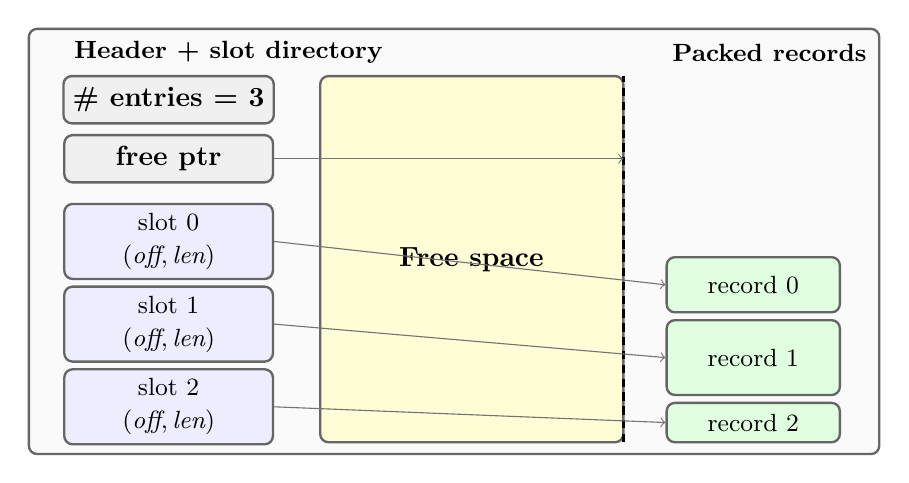
\begin{tikzpicture}[
    x=1cm,y=1cm,
    every node/.style={font=\small},
    frame/.style={draw=black!60, rounded corners=3pt, line width=0.85pt},
    header/.style={frame, fill=gray!12, minimum width=2.65cm, minimum height=0.6cm, align=center, font=\bfseries},
    slot/.style={frame, fill=blue!7, minimum width=2.65cm, minimum height=0.9cm, align=center},
    free/.style={frame, fill=yellow!16},
    rec/.style={frame, fill=green!12, minimum width=2.2cm, align=center},
    link/.style={->, thin, draw=black!55}
]
    \draw[frame, fill=gray!4] (0,0) rectangle (10.8,5.4);

    \node[anchor=west, font=\bfseries\small] at (0.45,5.10) {Header + slot directory};
    \node[anchor=west, font=\bfseries\small] at (8.05,5.10) {Packed records};

    \node[header] (h1) at (1.775,4.50) {\# entries = 3};
    \node[header] (h2) at (1.775,3.75) {free ptr};

    \node[slot] (s0) at (1.775,2.70) {slot 0\\[0.1em]$(\textit{off},\textit{len})$};
    \node[slot] (s1) at (1.775,1.65) {slot 1\\[0.1em]$(\textit{off},\textit{len})$};
    \node[slot] (s2) at (1.775,0.60) {slot 2\\[0.1em]$(\textit{off},\textit{len})$};

    \draw[free] (3.70,0.15) rectangle (7.55,4.80);
    \node[font=\bfseries] at (5.62,2.47) {Free space};
    \draw[densely dashed, line width=0.9pt] (7.55,0.15) -- (7.55,4.80);
    \draw[link] (h2.east) -- (7.55,3.75);

    \node[rec, minimum height=0.7cm] (r0) at (9.20,2.15) {record 0};
    \node[rec, minimum height=0.95cm] (r1) at (9.20,1.225) {record 1};
    \node[rec, minimum height=0.5cm] (r2) at (9.20,0.40) {record 2};

    \draw[link] (s0.east) -- (r0.west);
    \draw[link] (s1.east) -- (r1.west);
    \draw[link] (s2.east) -- (r2.west);
\end{tikzpicture}
}\par}
\end{figure}

The header and slot directory grow from the front of the page. The records grow from the back. A free-space pointer marks the boundary between them. During compaction, the DBMS can move the record bytes without changing the slot number, so the RID stays the same.

The header stores:
\begin{dashlist}
    \item the number of slot entries,
    \item a free-space pointer,
    \item one slot entry per record with its location and size.
\end{dashlist}

\subsubsection*{Operational issues}
\begin{dashlist}
    \item \textbf{record growth}: updating a field may force data to shift within the page,
    \item \textbf{page overflow}: if the record no longer fits, it may move to another page, often with a forwarding pointer,
    \item \textbf{oversized records}: some systems forbid records larger than a page, while others spill large values to overflow storage.
\end{dashlist}

\section{Row- and column-oriented layouts}
The page layouts above use the classic row-store design: each slot points to one full tuple. This is also called the \textbf{N-ary storage model (NSM)}.

\begin{concept}{Decomposition storage model (DSM)}
A column-oriented layout where each attribute is stored separately. To rebuild a tuple, the system reads the values at the same logical position from the needed columns.
\end{concept}

\begin{figure}[htp]
\centering
{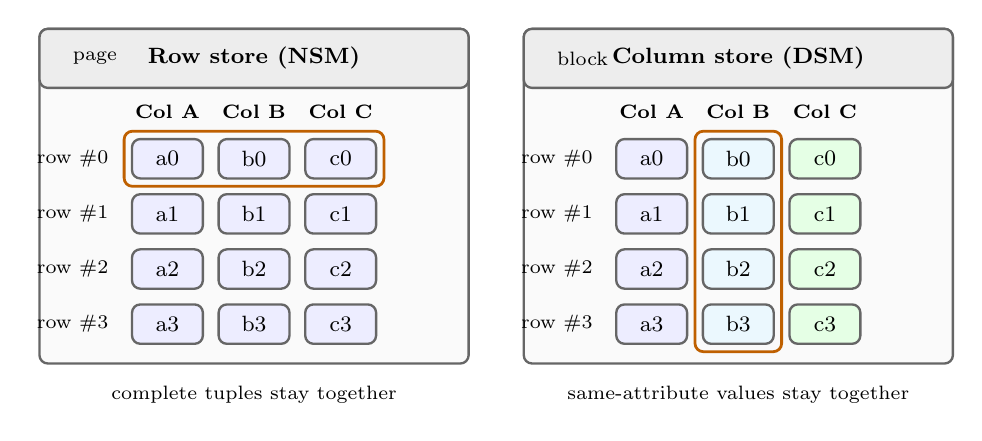
\begin{tikzpicture}[
    x=1cm,y=1cm,
    every node/.style={font=\footnotesize},
    frame/.style={draw=black!60, rounded corners=3pt, line width=0.85pt},
    header/.style={frame, fill=gray!14},
    cell/.style={frame, minimum width=0.90cm, minimum height=0.50cm, fill=blue!7},
    acol/.style={frame, minimum width=0.90cm, minimum height=0.50cm, fill=blue!7},
    bcol/.style={frame, minimum width=0.90cm, minimum height=0.50cm, fill=cyan!8},
    ccol/.style={frame, minimum width=0.90cm, minimum height=0.50cm, fill=green!10},
    accent/.style={draw=orange!75!black, rounded corners=3pt, line width=1.0pt}
]
    \draw[frame, fill=gray!4] (0,0) rectangle (5.45,4.25);
    \draw[header] (0,3.50) rectangle (5.45,4.25);
    \node[font=\footnotesize\bfseries] at (2.725,3.875) {Row store (NSM)};
    \node[font=\scriptsize, anchor=west] at (0.30,3.875) {page};

    \foreach \x/\lbl in {1.625/A, 2.725/B, 3.825/C} {
        \node[font=\scriptsize\bfseries] at (\x,3.20) {Col \lbl};
    }
    \foreach \r/\y in {0/2.60, 1/1.90, 2/1.20, 3/0.50} {
        \node[font=\scriptsize, anchor=east] at (1.00,\y) {row \#\r};
    }

    \node[cell] at (1.625,2.60) {a0};
    \node[cell] at (2.725,2.60) {b0};
    \node[cell] at (3.825,2.60) {c0};
    \node[cell] at (1.625,1.90) {a1};
    \node[cell] at (2.725,1.90) {b1};
    \node[cell] at (3.825,1.90) {c1};
    \node[cell] at (1.625,1.20) {a2};
    \node[cell] at (2.725,1.20) {b2};
    \node[cell] at (3.825,1.20) {c2};
    \node[cell] at (1.625,0.50) {a3};
    \node[cell] at (2.725,0.50) {b3};
    \node[cell] at (3.825,0.50) {c3};
    \draw[accent] (1.075,2.25) rectangle (4.375,2.95);

    \draw[frame, fill=gray!4] (6.15,0) rectangle (11.60,4.25);
    \draw[header] (6.15,3.50) rectangle (11.60,4.25);
    \node[font=\footnotesize\bfseries] at (8.875,3.875) {Column store (DSM)};
    \node[font=\scriptsize, anchor=west] at (6.45,3.875) {block};

    \foreach \x/\lbl in {7.775/A, 8.875/B, 9.975/C} {
        \node[font=\scriptsize\bfseries] at (\x,3.20) {Col \lbl};
    }
    \foreach \r/\y in {0/2.60, 1/1.90, 2/1.20, 3/0.50} {
        \node[font=\scriptsize, anchor=east] at (7.15,\y) {row \#\r};
    }

    \node[acol] at (7.775,2.60) {a0};
    \node[acol] at (7.775,1.90) {a1};
    \node[acol] at (7.775,1.20) {a2};
    \node[acol] at (7.775,0.50) {a3};

    \node[bcol] at (8.875,2.60) {b0};
    \node[bcol] at (8.875,1.90) {b1};
    \node[bcol] at (8.875,1.20) {b2};
    \node[bcol] at (8.875,0.50) {b3};

    \node[ccol] at (9.975,2.60) {c0};
    \node[ccol] at (9.975,1.90) {c1};
    \node[ccol] at (9.975,1.20) {c2};
    \node[ccol] at (9.975,0.50) {c3};
    \draw[accent] (8.325,0.15) rectangle (9.425,2.95);

    \node[font=\scriptsize] at (2.725,-0.40) {complete tuples stay together};
    \node[font=\scriptsize] at (8.875,-0.40) {same-attribute values stay together};
\end{tikzpicture}
}\par}
\end{figure}

\subsection{Row store versus column store}
Row stores keep all attributes of a tuple together. They work well when queries read or update whole records.
\begin{dashlist}
    \item \textbf{row-store advantages}: fast inserts, updates, and deletes; good when workloads read or rewrite full tuples; works well with clustered, index-based storage.
    \item \textbf{row-store disadvantages}: inefficient when a query scans many tuples but needs only a few attributes; compression is weaker because one page mixes many value types.
\end{dashlist}

Column stores make the opposite trade-off. They optimize scans over attributes instead of full tuples.
\begin{dashlist}
    \item \textbf{column-store advantages}: reduced I/O when only some attributes are needed, better CPU cache locality, stronger compression, and efficient vectorized processing.
    \item \textbf{column-store disadvantages}: full-tuple reconstruction is expensive, updates and deletions are harder, and compressed data may need decompression before processing.
\end{dashlist}

As a rule of thumb, \textbf{row stores} fit transactional workloads (\textbf{OLTP}), while \textbf{column stores} fit analytical workloads (\textbf{OLAP}). Some systems support both and act as \textbf{hybrid row/column stores}.

\subsection{Partition Attributes Across (PAX)}
Pure column stores separate attributes across the whole file. \textbf{PAX} is a middle ground: from the outside the page still looks like a row-store page, but inside the page the values are grouped by column.

\begin{concept}{PAX}
Within one page, values of the same attribute are stored together in column partitions. A tuple is rebuilt logically by taking the same offset in each partition.
\end{concept}

\begin{figure}[htp]
\centering
{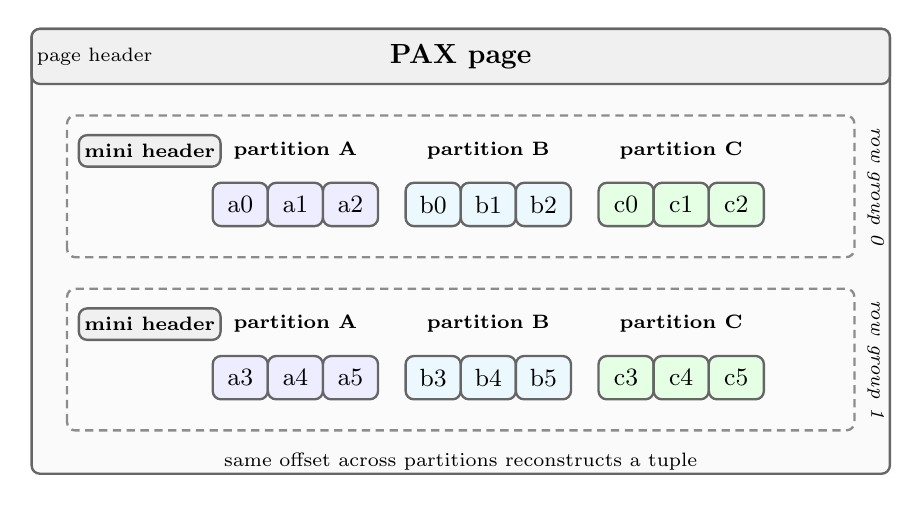
\begin{tikzpicture}[
    x=1cm,y=1cm,
    every node/.style={font=\small},
    frame/.style={draw=black!60, rounded corners=3pt, line width=0.85pt},
    header/.style={frame, fill=gray!12},
    group/.style={draw=black!45, rounded corners=3pt, line width=0.85pt, densely dashed, fill=gray!3},
    acell/.style={frame, minimum width=0.70cm, minimum height=0.55cm, fill=blue!7},
    bcell/.style={frame, minimum width=0.70cm, minimum height=0.55cm, fill=cyan!8},
    ccell/.style={frame, minimum width=0.70cm, minimum height=0.55cm, fill=green!10}
]
    \draw[frame, fill=gray!4] (0,0) rectangle (10.9,5.65);
    \draw[header] (0,4.95) rectangle (10.9,5.65);
    \node[font=\bfseries] at (5.45,5.30) {PAX page};
    \node[font=\scriptsize] at (0.80,5.30) {page header};

    \draw[group] (0.45,2.75) rectangle (10.45,4.55);
    \draw[group] (0.45,0.55) rectangle (10.45,2.35);

    \draw[header] (0.60,3.90) rectangle (2.40,4.30);
    \draw[header] (0.60,1.70) rectangle (2.40,2.10);
    \node[font=\bfseries] at (1.50,4.10) {\scriptsize mini header};
    \node[font=\bfseries] at (1.50,1.90) {\scriptsize mini header};

    \foreach \x/\lbl in {3.35/A,5.80/B,8.25/C} {
        \node[font=\scriptsize\bfseries] at (\x,4.10) {partition \lbl};
        \node[font=\scriptsize\bfseries] at (\x,1.90) {partition \lbl};
    }

    \node[acell] at (2.65,3.42) {a0};
    \node[acell] at (3.35,3.42) {a1};
    \node[acell] at (4.05,3.42) {a2};
    \node[bcell] at (5.10,3.42) {b0};
    \node[bcell] at (5.80,3.42) {b1};
    \node[bcell] at (6.50,3.42) {b2};
    \node[ccell] at (7.55,3.42) {c0};
    \node[ccell] at (8.25,3.42) {c1};
    \node[ccell] at (8.95,3.42) {c2};

    \node[acell] at (2.65,1.22) {a3};
    \node[acell] at (3.35,1.22) {a4};
    \node[acell] at (4.05,1.22) {a5};
    \node[bcell] at (5.10,1.22) {b3};
    \node[bcell] at (5.80,1.22) {b4};
    \node[bcell] at (6.50,1.22) {b5};
    \node[ccell] at (7.55,1.22) {c3};
    \node[ccell] at (8.25,1.22) {c4};
    \node[ccell] at (8.95,1.22) {c5};

    \node[font=\scriptsize\itshape, rotate=-90] at (10.72,3.65) {row group 0};
    \node[font=\scriptsize\itshape, rotate=-90] at (10.72,1.45) {row group 1};
    \node[font=\scriptsize] at (5.45,0.15) {same offset across partitions reconstructs a tuple};
\end{tikzpicture}
}\par}
\end{figure}

A PAX page keeps:
\begin{dashlist}
    \item the same number of tuples per page as a traditional row page,
    \item one contiguous partition per attribute inside the page,
    \item logical rather than physical row boundaries.
\end{dashlist}

This improves cache behavior for scans over a few attributes without giving up the page-based design already used by row stores.

\subsection{Columnar file formats}
Modern analytical file formats apply the same idea at the file level. Formats such as \textbf{Parquet} and \textbf{ORC} group tuples into large row groups (or stripes) and store each group column by column.

\begin{figure}[htp]
\centering
{\begin{tikzpicture}[
    x=1cm,y=1cm,
    scale=0.94,
    transform shape,
    every node/.style={font=\small},
    >=Latex,
    frame/.style={draw=black!60, rounded corners=3pt, line width=0.85pt},
    meta/.style={frame, fill=gray!12},
    rowdata/.style={frame, fill=blue!7},
    footer/.style={frame, fill=yellow!18},
    colindex/.style={frame, fill=cyan!10, minimum width=2.35cm, minimum height=0.58cm},
    coldata/.style={frame, fill=green!10, minimum width=2.35cm, minimum height=0.58cm},
    link/.style={->, thin, draw=black!55}
]
    \node[font=\bfseries] at (2.15,7.65) {File of row groups / stripes};
    \node[font=\bfseries] at (8.25,7.65) {Inside one stripe};

    \draw[frame, fill=gray!4] (0.35,5.35) rectangle (3.95,7.15);
    \draw[meta]   (0.35,6.55) rectangle (3.95,7.15);
    \draw[rowdata](0.35,5.95) rectangle (3.95,6.55);
    \draw[footer] (0.35,5.35) rectangle (3.95,5.95);
    \node[anchor=east] at (0.10,6.25) {stripe 1};
    \node at (2.15,6.85) {Index data};
    \node at (2.15,6.25) {Row data};
    \node at (2.15,5.65) {Stripe footer};

    \draw[frame, fill=gray!4] (0.35,3.10) rectangle (3.95,4.90);
    \draw[meta]   (0.35,4.30) rectangle (3.95,4.90);
    \draw[rowdata](0.35,3.70) rectangle (3.95,4.30);
    \draw[footer] (0.35,3.10) rectangle (3.95,3.70);
    \node[anchor=east] at (0.10,4.00) {stripe 2};
    \node (idxsrc) at (2.15,4.60) {Index data};
    \node (rowsrc) at (2.15,4.00) {Row data};
    \node at (2.15,3.40) {Stripe footer};

    \node at (2.15,2.55) {$\vdots$};

    \draw[frame, fill=gray!4] (0.35,0.40) rectangle (3.95,2.20);
    \draw[meta]   (0.35,1.60) rectangle (3.95,2.20);
    \draw[rowdata](0.35,1.00) rectangle (3.95,1.60);
    \draw[footer] (0.35,0.40) rectangle (3.95,1.00);
    \node[anchor=east] at (0.10,1.30) {stripe $n$};
    \node at (2.15,1.90) {Index data};
    \node at (2.15,1.30) {Row data};
    \node at (2.15,0.70) {Stripe footer};

    \draw[footer] (0.35,-0.55) rectangle (3.95,0.05);
    \node at (2.15,-0.25) {File footer};

    \node[colindex] (i1) at (8.25,5.45) {Col 1 index};
    \node[colindex] (i2) at (8.25,4.70) {Col 2 index};
    \node[colindex] (i3) at (8.25,3.95) {Col 3 index};

    \node[coldata] (d1) at (8.25,2.70) {Col 1 data};
    \node[coldata] (d2) at (8.25,1.95) {Col 2 data};
    \node[coldata] (d3) at (8.25,1.20) {Col 3 data};

    \draw[link] (3.95,4.60) -- (i1.west);
    \draw[link] (3.95,4.60) -- (i2.west);
    \draw[link] (3.95,4.60) -- (i3.west);
    \draw[link] (3.95,4.00) -- (d1.west);
    \draw[link] (3.95,4.00) -- (d2.west);
    \draw[link] (3.95,4.00) -- (d3.west);

    \node[font=\scriptsize] at (8.25,0.35) {metadata and column streams are stored separately};
\end{tikzpicture}
}\par}
\end{figure}

These formats are popular in big-data systems because:
\begin{dashlist}
    \item each column stream compresses well,
    \item the engine can skip irrelevant columns and often entire groups,
    \item scans over a subset of attributes avoid touching the rest of the file.
\end{dashlist}

\section{Alternative file organizations}
So far, we looked at how records are stored \emph{inside} pages. Another design choice is how pages are arranged \emph{inside} a file.

\begin{dashlist}
    \item \textbf{heap files}: good when typical access is a full file scan or when insertion simplicity matters most,
    \item \textbf{sorted files}: good when records are often read in order or by key range,
    \item \textbf{index-based organizations}: discussed in the indexing part.
\end{dashlist}

\subsection{Heap files}
\begin{concept}{Heap file}
An unordered file organization: records are stored in no particular search order.
\end{concept}

Heap files are the simplest file organization.
\begin{dashlist}
    \item records can be scanned sequentially, or accessed directly if their RID is known,
    \item inserts place a new record in any page with enough free space,
    \item as the file grows or shrinks, pages are allocated and deallocated, so the DBMS must track free space.
\end{dashlist}

The DBMS usually finds heap pages in one of two ways:
\begin{dashlist}
    \item \textbf{linked lists}: a header page points to a list of free pages and a list of data pages,
    \item \textbf{page directories}: directory pages store each data page location together with its remaining free space.
\end{dashlist}

\begin{figure}[htp]
\centering
{\begin{tikzpicture}[
    x=1cm,y=1cm,
    every node/.style={font=\small},
    >=Latex,
    frame/.style={draw=black!60, rounded corners=3pt, line width=0.85pt},
    header/.style={frame, fill=gray!12},
    entry/.style={frame, fill=blue!7, minimum width=2.6cm, minimum height=0.56cm},
    used/.style={frame, fill=green!10},
    free/.style={frame, fill=yellow!18},
    link/.style={->, thick, draw=black!55}
]
    % Directory
    \draw[frame, fill=gray!4] (0,0.55) rectangle (3.00,4.45);
    \draw[header] (0,3.70) rectangle (3.00,4.45);
    \node[font=\bfseries] at (1.50,4.08) {Directory};
    \node[entry] (e0) at (1.50,3.05) {P42 | 20\% free};
    \node[entry] (e1) at (1.50,2.20) {P43 | \phantom{0}0\% free};
    \node[entry] (e2) at (1.50,1.35) {P44 | 55\% free};
    \node at (1.50,0.85) {$\vdots$};

    % Page 42
    \draw[frame, fill=gray!4] (4.00,0.95) rectangle (5.80,4.05);
    \draw[header] (4.00,3.45) rectangle (5.80,4.05);
    \draw[used]   (4.20,1.15) rectangle (5.60,2.83);
    \draw[free]   (4.20,2.83) rectangle (5.60,3.25);
    \node[font=\bfseries] at (4.90,3.75) {Page 42};
    \node[font=\scriptsize] at (4.90,1.99) {data};
    \node[font=\scriptsize] at (4.90,3.04) {free};

    % Page 43
    \draw[frame, fill=gray!4] (6.60,0.95) rectangle (8.40,4.05);
    \draw[header] (6.60,3.45) rectangle (8.40,4.05);
    \draw[used]   (6.80,1.15) rectangle (8.20,3.25);
    \node[font=\bfseries] at (7.50,3.75) {Page 43};
    \node[font=\scriptsize] at (7.50,2.20) {full};

    % Page 44
    \draw[frame, fill=gray!4] (9.20,0.95) rectangle (11.00,4.05);
    \draw[header] (9.20,3.45) rectangle (11.00,4.05);
    \draw[used]   (9.40,1.15) rectangle (10.80,2.10);
    \draw[free]   (9.40,2.10) rectangle (10.80,3.25);
    \node[font=\bfseries] at (10.10,3.75) {Page 44};
    \node[font=\scriptsize] at (10.10,1.62) {data};
    \node[font=\scriptsize] at (10.10,2.67) {free};

    % Links
    \draw[link, rounded corners=5pt] (e0.east) -- (4.00,3.05);
    \draw[link, rounded corners=5pt] (e1.east) -- (3.50,2.20) -- (3.50,0.60) -- (7.50,0.60) -- (7.50,0.95);
    \draw[link, rounded corners=5pt] (e2.east) -- (3.20,1.35) -- (3.20,0.40) -- (10.10,0.40) -- (10.10,0.95);

    % Caption text
    \node[font=\footnotesize, text=black!80] at (5.50,-0.30) {directory entry = page id + free-space summary};
\end{tikzpicture}
}\par}
\end{figure}

Heap files work well when most queries scan the file, because the DBMS does not maintain physical order.
\newpage
\subsection{Sorted (sequential) files}
\begin{concept}{Search key}
Attributes used to physically order records in a sorted file. They may be unique, but they do not have to be.
\end{concept}

In a sorted file, records appear in search-key order.
\begin{dashlist}
    \item this is good for scanning the whole file in order,
    \item range queries are efficient because, after the first match, the DBMS can keep reading forward in order.
\end{dashlist}

\begin{figure}[htp]
\centering
{\begin{tikzpicture}[
    x=1cm,y=1cm,
    every node/.style={font=\small},
    >=Latex,
    frame/.style={draw=black!60, rounded corners=3pt, line width=0.85pt},
    header/.style={frame, fill=gray!12},
    rec/.style={frame, fill=blue!7, minimum width=1.95cm, minimum height=0.55cm},
    overrec/.style={frame, fill=orange!14, minimum width=1.95cm, minimum height=0.55cm},
    link/.style={->, thick, draw=black!55}
]
    \draw[frame, fill=gray!4] (0.10,0.90) rectangle (3.15,4.15);
    \draw[header] (0.10,3.55) rectangle (3.15,4.15);
    \node[font=\bfseries] at (1.62,3.85) {Page 0};
    \node[rec] (r10) at (1.62,2.95) {10};
    \node[rec] (r20) at (1.62,2.10) {20};
    \node[rec] (r30) at (1.62,1.25) {30};

    \draw[frame, fill=gray!4] (4.25,0.90) rectangle (7.30,4.15);
    \draw[header] (4.25,3.55) rectangle (7.30,4.15);
    \node[font=\bfseries] at (5.78,3.85) {Page 1};
    \node[rec] (r40) at (5.78,2.95) {40};
    \node[rec] (r50) at (5.78,2.10) {50};
    \node[rec] (r60) at (5.78,1.25) {60};

    \draw[frame, fill=gray!4] (1.95,-0.55) rectangle (5.45,0.55);
    \draw[header] (1.95,0.00) rectangle (5.45,0.55);
    \node[font=\bfseries] at (3.70,0.27) {Overflow block};
    \node[overrec] (r35) at (3.70,-0.33) {35};

    \draw[link] (r30.south) to[out=-70,in=180] (r35.west);
    \draw[link] (r35.east) to[out=0,in=-120] (r40.south);

    \node[font=\scriptsize] at (3.70,4.55) {records remain ordered by the search key};
    \node[font=\scriptsize] at (3.70,-1.00) {if the target page is full, insert into overflow and update the chain};
\end{tikzpicture}
}\par}
\end{figure}

Keeping that order makes updates more expensive:
\begin{dashlist}
    \item \textbf{deletion}: systems often use pointer chains or tombstones so later records do not need to move right away,
    \item \textbf{insertion}: the DBMS finds the right position; if the target page has room, it inserts there, otherwise it uses an overflow page and updates the chain,
    \item over time, overflow pages accumulate, so the file must sometimes be reorganized to restore physical order.
\end{dashlist}

\subsection{Heap files versus sorted files}
Which organization is better depends on the workload. Heap files make updates cheap. Sorted files make ordered search cheap. To compare them, we use a simple cost model.

\begin{concept}{Simplified I/O cost model}
Measure cost only in page I/Os. In this model, I/O dominates CPU work, so we ignore buffering, prefetching, and other system effects. We also focus only on the average case.
\end{concept}

Assumptions:
\begin{dashlist}
    \item $B$ is the number of data pages in the file.
    \item Each operation inserts or deletes a single record.
    \item An equality search returns exactly one matching record.
    \item In a heap file, insertion appends at the end of the file.
    \item In a sorted file, searches use the file-ordering attribute and deletions keep the file compacted.
\end{dashlist}

\begin{figure}[htp]
\centering
{{\small
\setlength{\tabcolsep}{6pt}
\renewcommand{\arraystretch}{1.2}
\arrayrulecolor{black!60}
\begin{adjustbox}{max width=\textwidth}
\begin{tabular}{|L{3.1cm}|C{2.0cm}|C{4.0cm}|L{4.5cm}|}
\hline
\rowcolor{gray!14}
\textbf{Operation} & \textbf{Heap file} & \textbf{Sorted file} & \textbf{Notes} \\
\hline
Scan all records & $B$ & $B$ & $B$ = \# of data pages \\
\hline
Equality search & $0.5B$ & $\log_2 B$ & assumes exactly one matching record \\
\hline
Range search & $B$ & $\log_2 B + \#\text{match pages}$ & after the first match, keep reading forward \\
\hline
Insert & $2$ & $\log_2 B + 2\cdot(B/2)$ & must read and rewrite about half the file \\
\hline
Delete & $0.5B + 1$ & $\log_2 B + 2\cdot(B/2)$ & search first, then pay the same shifting cost \\
\hline
\end{tabular}
\end{adjustbox}
}
}\par}
\end{figure}

The main trade-off is:
\begin{dashlist}
    \item scans cost about the same in both organizations,
    \item sorted files are much better for equality and range search on the ordering attribute,
    \item heap files are much better for inserts and usually for deletes, because they avoid shifting many records.
\end{dashlist}

A sorted file gives one very good access path, but it pays heavily for updates. This is why indexes are useful.

\section{Indexing}
A sorted file helps only for one physical order. If the file is sorted on \texttt{ID}, then lookups on \texttt{ID} are efficient, but predicates on \texttt{salary} or \texttt{dept\_name} may still need a scan.

\begin{concept}{Index}
An auxiliary access structure that maps search-key values to records or pages, so the DBMS can answer selections with fewer I/Os than a full file scan.
\end{concept}

\begin{figure}[htp]
\centering
{\begin{tikzpicture}[
    x=1cm,y=1cm,
    every node/.style={font=\small},
    >=Latex,
    frame/.style={draw=black!60, rounded corners=3pt, line width=0.85pt},
    header/.style={frame, fill=gray!12},
    idxframe/.style={frame, fill=gray!4},
    idxentry/.style={frame, fill=orange!14, minimum width=2.10cm, minimum height=0.46cm, font=\scriptsize},
    link/.style={->, thick, draw=orange!75!black}
]
    \draw[frame, fill=blue!3] (4.25,0.25) rectangle (12.35,5.05);
    \draw[header] (4.25,4.45) rectangle (12.35,5.05);
    \foreach \x in {5.75,7.95,10.45} {
        \draw[black!45] (\x,0.25) -- (\x,5.05);
    }
    \foreach \y in {3.75,3.05,2.35,1.65,0.95} {
        \draw[black!45] (4.25,\y) -- (12.35,\y);
    }

    \node[font=\scriptsize\bfseries] at (5.00,4.75) {ID};
    \node[font=\scriptsize\bfseries] at (6.85,4.75) {name};
    \node[font=\scriptsize\bfseries] at (9.20,4.75) {dept\_name};
    \node[font=\scriptsize\bfseries] at (11.40,4.75) {salary};

    \node[font=\scriptsize] at (5.00,4.10) {10101};
    \node[font=\scriptsize] at (6.85,4.10) {Srinivasan};
    \node[font=\scriptsize] at (9.20,4.10) {Comp.\ Sci.};
    \node[font=\scriptsize] at (11.40,4.10) {65000};

    \node[font=\scriptsize] at (5.00,3.40) {12121};
    \node[font=\scriptsize] at (6.85,3.40) {Wu};
    \node[font=\scriptsize] at (9.20,3.40) {Finance};
    \node[font=\scriptsize] at (11.40,3.40) {90000};

    \node[font=\scriptsize] at (5.00,2.70) {22222};
    \node[font=\scriptsize] at (6.85,2.70) {Einstein};
    \node[font=\scriptsize] at (9.20,2.70) {Physics};
    \node[font=\scriptsize] at (11.40,2.70) {95000};

    \node[font=\scriptsize] at (5.00,2.00) {33456};
    \node[font=\scriptsize] at (6.85,2.00) {Gold};
    \node[font=\scriptsize] at (9.20,2.00) {Physics};
    \node[font=\scriptsize] at (11.40,2.00) {87000};

    \node[font=\scriptsize] at (5.00,1.30) {83821};
    \node[font=\scriptsize] at (6.85,1.30) {Brandt};
    \node[font=\scriptsize] at (9.20,1.30) {Comp.\ Sci.};
    \node[font=\scriptsize] at (11.40,1.30) {92000};

    \node[font=\scriptsize] at (5.00,0.60) {98345};
    \node[font=\scriptsize] at (6.85,0.60) {Kim};
    \node[font=\scriptsize] at (9.20,0.60) {Elec.\ Eng.};
    \node[font=\scriptsize] at (11.40,0.60) {80000};

    \draw[idxframe] (0.25,2.85) rectangle (3.45,5.15);
    \draw[header] (0.25,4.55) rectangle (3.45,5.15);
    \node[font=\scriptsize\bfseries] at (1.85,4.85) {Index on ID};
    \node[idxentry] (id22222) at (1.85,4.24) {22222};
    \node[idxentry] (id33456) at (1.85,3.70) {33456};
    \node[idxentry] (id83821) at (1.85,3.16) {83821};

    \draw[idxframe] (0.25,0.15) rectangle (3.45,2.45);
    \draw[header] (0.25,1.85) rectangle (3.45,2.45);
    \node[font=\scriptsize\bfseries] at (1.85,2.15) {Index on Salary};
    \node[idxentry] (sal90000) at (1.85,1.54) {90000};
    \node[idxentry] (sal92000) at (1.85,1.00) {92000};
    \node[idxentry] (sal95000) at (1.85,0.46) {95000};

    \draw[link] (id22222.east) -- (4.25,2.70);
    \draw[link] (id33456.east) -- (4.25,2.00);
    \draw[link] (id83821.east) -- (4.25,1.30);

    \draw[link] (sal90000.east) -- (4.25,3.40);
    \draw[link] (sal92000.east) -- (4.25,1.30);
    \draw[link] (sal95000.east) -- (4.25,2.70);

    \node[font=\scriptsize] at (8.30,-0.18) {one physical order, multiple efficient access paths};
\end{tikzpicture}
}\par}
\end{figure}

Indexes matter because:
\begin{dashlist}
    \item they give the same relation several efficient access paths,
    \item they speed up selections on the index's search-key fields,
    \item the search key does not need to be unique,
    \item any subset of relation attributes can be used as a search key,
    \item inserts, deletes, and updates must also maintain the affected indexes.
\end{dashlist}

\subsection{Index search conditions}
\begin{concept}{Index search condition}
A predicate of the form $\langle \text{search key}, \text{comparison operator} \rangle$.
\end{concept}

Examples:
\begin{dashlist}
    \item \textbf{\texttt{dept\_name = "CS"}}: search key = \texttt{dept\_name}, operator = equality.
    \item \textbf{\texttt{gpa > 3}}: search key = \texttt{gpa}, operator = greater-than.
\end{dashlist}

Equality predicates ask for one exact key value. Inequality predicates such as $<$, $\leq$, $>$, and $\geq$ define ranges, so they benefit most from ordered access paths.

\section{Index classification}
Indexes are commonly described along four independent axes:
\begin{dashlist}
    \item \textbf{clustered vs. unclustered},
    \item \textbf{dense vs. sparse},
    \item \textbf{key vs. non-key search key},
    \item \textbf{data file ordered vs. not ordered on the indexing field}.
\end{dashlist}

\subsection{Clustered and unclustered indexes}
\begin{concept}{Clustered vs. unclustered}
If the physical order of the data records follows the order of the index entries, the index is \textbf{clustered}. Otherwise it is \textbf{unclustered}.
\end{concept}

\begin{figure}[htp]
\centering
{\begin{tikzpicture}[
    x=1cm,y=1cm,
    every node/.style={font=\small},
    >=Latex,
    frame/.style={draw=black!60, rounded corners=3pt, line width=0.85pt},
    idx/.style={frame, fill=orange!14, minimum width=1.15cm, minimum height=0.62cm},
    data/.style={frame, fill=blue!7, minimum width=0.92cm, minimum height=0.62cm},
    link/.style={->, thick, draw=black!55}
]
    \node[font=\bfseries] at (3.40,4.45) {Clustered};
    \node[font=\bfseries] at (10.60,4.45) {Unclustered};

    \node[idx] (c10) at (1.40,3.35) {10};
    \node[idx] (c20) at (3.40,3.35) {20};
    \node[idx] (c30) at (5.40,3.35) {30};

    \node[data] (cd1) at (0.90,1.15) {10};
    \node[data] (cd2) at (1.90,1.15) {12};
    \node[data] (cd3) at (2.90,1.15) {20};
    \node[data] (cd4) at (3.90,1.15) {22};
    \node[data] (cd5) at (4.90,1.15) {30};
    \node[data] (cd6) at (5.90,1.15) {32};

    \draw[link] (c10.south) -- (cd1.north);
    \draw[link] (c10.south) -- (cd2.north);
    \draw[link] (c20.south) -- (cd3.north);
    \draw[link] (c20.south) -- (cd4.north);
    \draw[link] (c30.south) -- (cd5.north);
    \draw[link] (c30.south) -- (cd6.north);

    \node[idx] (u10) at (8.60,3.35) {10};
    \node[idx] (u20) at (10.60,3.35) {20};
    \node[idx] (u30) at (12.60,3.35) {30};

    \node[data] (ud1) at (8.10,1.15) {22};
    \node[data] (ud2) at (9.10,1.15) {10};
    \node[data] (ud3) at (10.10,1.15) {30};
    \node[data] (ud4) at (11.10,1.15) {20};
    \node[data] (ud5) at (12.10,1.15) {12};
    \node[data] (ud6) at (13.10,1.15) {32};

    \draw[link] (u10.south) -- (ud2.north);
    \draw[link] (u10.south) -- (ud5.north);
    \draw[link] (u20.south) -- (ud1.north);
    \draw[link] (u20.south) -- (ud4.north);
    \draw[link] (u30.south) -- (ud3.north);
    \draw[link] (u30.south) -- (ud6.north);

    \draw[black!30] (0.35,2.25) -- (6.45,2.25);
    \draw[black!30] (7.55,2.25) -- (13.45,2.25);

    \node[font=\scriptsize] at (3.40,0.25) {nearby index entries lead to nearby data};
    \node[font=\scriptsize] at (10.60,0.25) {matching records are scattered across the file};
\end{tikzpicture}
}\par}
\end{figure}

This difference matters because:
\begin{dashlist}
    \item a clustered index keeps matching records on nearby pages, so range queries are efficient,
    \item an unclustered index may jump to many unrelated pages, so large result sets become expensive,
    \item a file can have many unclustered indexes, but only one clustered physical order at a time.
\end{dashlist}

Some textbooks use \emph{primary} for clustered and \emph{secondary} for unclustered indexes. That vocabulary is not universal across DBMSs, so the physical term \emph{clustered} is safer.

\begin{figure}[htp]
\centering
{\begin{tikzpicture}[
    x=1cm,y=1cm,
    every node/.style={font=\small},
    >=Latex,
    frame/.style={draw=black!60, rounded corners=3pt, line width=0.85pt},
    idx/.style={frame, fill=orange!14, minimum width=0.95cm, minimum height=0.5cm, font=\scriptsize},
    link/.style={->, thick, draw=black!55},
    page/.style={inner sep=0pt, outer sep=0pt}
]
    \node[idx] (e10101) at (0.75,3.35) {10101};
    \node[idx] (e12121) at (1.85,3.35) {12121};
    \node[idx] (e15151) at (3.05,3.35) {15151};
    \node[idx] (e22222) at (4.15,3.35) {22222};
    \node[font=\large] at (8.20,3.35) {$\cdots$};
    \node[idx] (e83821) at (12.25,3.35) {83821};
    \node[idx] (e98345) at (13.35,3.35) {98345};

    \draw[black!30] (0.00,2.20) -- (14.10,2.20);

    \node[page] (p0) at (1.30,0.78) {{
        \setlength{\tabcolsep}{3pt}
        \tiny
        \begin{tabular}{|C{0.6cm}|L{1.1cm}|}
        \hline
        10101 & Srinivasan\\
        \hline
        12121 & Wu\\
        \hline
        \end{tabular}
    }};

    \node[page] (p1) at (3.60,0.78) {{
        \setlength{\tabcolsep}{3pt}
        \tiny
        \begin{tabular}{|C{0.6cm}|L{1.1cm}|}
        \hline
        15151 & Mozart\\
        \hline
        22222 & Einstein\\
        \hline
        \end{tabular}
    }};

    \node[page] (p2) at (5.90,0.78) {{
        \setlength{\tabcolsep}{3pt}
        \tiny
        \begin{tabular}{|C{0.6cm}|L{1.1cm}|}
        \hline
        32343 & El Said\\
        \hline
        33456 & Gold\\
        \hline
        \end{tabular}
    }};

    \node[page] (p3) at (8.20,0.78) {{
        \setlength{\tabcolsep}{3pt}
        \tiny
        \begin{tabular}{|C{0.6cm}|L{1.1cm}|}
        \hline
        45565 & Katz\\
        \hline
        58583 & Califieri\\
        \hline
        \end{tabular}
    }};

    \node[page] (p4) at (10.50,0.78) {{
        \setlength{\tabcolsep}{3pt}
        \tiny
        \begin{tabular}{|C{0.6cm}|L{1.1cm}|}
        \hline
        76543 & Singh\\
        \hline
        76766 & Crick\\
        \hline
        \end{tabular}
    }};

    \node[page] (p5) at (12.80,0.78) {{
        \setlength{\tabcolsep}{3pt}
        \tiny
        \begin{tabular}{|C{0.6cm}|L{1.1cm}|}
        \hline
        83821 & Brandt\\
        \hline
        98345 & Kim\\
        \hline
        \end{tabular}
    }};

    \draw[link] (e10101.south) -- ([xshift=-0.25cm]p0.north);
    \draw[link] (e12121.south) -- ([xshift=0.25cm]p0.north);
    \draw[link] (e15151.south) -- ([xshift=-0.25cm]p1.north);
    \draw[link] (e22222.south) -- ([xshift=0.25cm]p1.north);
    \draw[link] (e83821.south) -- ([xshift=-0.25cm]p5.north);
    \draw[link] (e98345.south) -- ([xshift=0.25cm]p5.north);

    \node[font=\scriptsize] at (7.05,-0.15) {clustered index on \texttt{ID}: nearby index entries point to nearby data pages};
\end{tikzpicture}
}\par}
\end{figure}

In the example above, the data file is ordered on \texttt{ID}. Nearby index entries lead to nearby data pages, which is exactly the clustered case.

\subsection{Dense and sparse indexes}
\begin{concept}{Dense index}
Has an index entry for every search-key value that appears in the data file.
\end{concept}

\begin{concept}{Sparse index}
Has entries for only some search-key values, usually one entry per data page or page range.
\end{concept}

A sparse index uses less space and needs fewer updates, but it works well only when the data file is ordered on the search key. After the sparse index points to the right page, the DBMS still searches within that page.

\subsubsection*{Range scans: why clustering matters}
For range predicates, the difference between clustered and unclustered indexes becomes much larger:
\begin{dashlist}
    \item with a \textbf{clustered} index, cost is roughly the number of \textbf{data pages} containing matching records,
    \item with an \textbf{unclustered} index, cost is closer to the number of \textbf{matching index entries}, because each match may lead to a different data page.
\end{dashlist}

So the trade-off is:
\begin{dashlist}
    \item \textbf{clustered advantage}: very efficient for range queries and ordered scans,
    \item \textbf{clustered drawback}: expensive to maintain, because updates disturb the physical order,
    \item \textbf{unclustered advantage}: easy to add as an extra access path without reorganizing the data file,
    \item \textbf{unclustered drawback}: large result sets can cause many random I/Os.
\end{dashlist}

\subsubsection*{Dense index on a key attribute}
If the search key is a key, each value identifies one record. Then a dense index has one entry per record, and each entry can point directly to one RID.

\begin{figure}[htp]
\centering
{\resizebox{0.92\textwidth}{!}{\begin{tikzpicture}[
    x=1cm,y=1cm,
    every node/.style={font=\small},
    >=Latex,
    frame/.style={draw=black!60, rounded corners=3pt, line width=0.85pt},
    header/.style={frame, fill=gray!12},
    idxentry/.style={frame, fill=orange!14, minimum width=2.25cm, minimum height=0.40cm},
    link/.style={->, thick, draw=black!50}
]
    \draw[frame, fill=gray!4] (0.10,0.25) rectangle (3.15,6.45);
    \draw[header] (0.10,5.90) rectangle (3.15,6.45);
    \node[font=\bfseries] at (1.62,6.18) {\small Dense index};

    \foreach \y/\v in {
        5.67/10101,
        5.20/12121,
        4.73/15151,
        4.26/22222,
        3.79/32343,
        3.32/33456,
        2.85/45565,
        2.38/58583,
        1.91/76543,
        1.44/76766,
        0.97/83821,
        0.50/98345
    }{
        \node[idxentry] at (1.62,\y) {\scriptsize \v};
    }

    \draw[frame, fill=blue!4] (4.05,0.25) rectangle (13.15,6.45);
    \draw[header] (4.05,5.90) rectangle (13.15,6.45);
    \foreach \x in {5.35,7.45,10.45} {
        \draw[black!45] (\x,0.25) -- (\x,6.45);
    }
    \foreach \y in {5.43,4.96,4.49,4.02,3.55,3.08,2.61,2.14,1.67,1.20,0.73,0.26} {
        \draw[black!40] (4.05,\y) -- (13.15,\y);
    }

    \node[font=\scriptsize\bfseries] at (4.70,6.18) {ID};
    \node[font=\scriptsize\bfseries] at (6.40,6.18) {name};
    \node[font=\scriptsize\bfseries] at (8.95,6.18) {dept\_name};
    \node[font=\scriptsize\bfseries] at (11.80,6.18) {salary};

    \foreach \y/\id/\name/\dept/\salary in {
        5.67/10101/Srinivasan/Comp.\ Sci./65000,
        5.20/12121/Wu/Finance/90000,
        4.73/15151/Mozart/Music/40000,
        4.26/22222/Einstein/Physics/95000,
        3.79/32343/El Said/History/60000,
        3.32/33456/Gold/Physics/87000,
        2.85/45565/Katz/Comp.\ Sci./75000,
        2.38/58583/Califieri/History/62000,
        1.91/76543/Singh/Finance/80000,
        1.44/76766/Crick/Biology/72000,
        0.97/83821/Brandt/Comp.\ Sci./92000,
        0.50/98345/Kim/Elec.\ Eng./80000
    }{
        \node[font=\scriptsize] at (4.70,\y) {\id};
        \node[font=\scriptsize] at (6.40,\y) {\name};
        \node[font=\scriptsize] at (8.95,\y) {\dept};
        \node[font=\scriptsize] at (11.80,\y) {\salary};
        \draw[link] (2.78,\y) -- (4.05,\y);
    }

    \node[font=\scriptsize] at (6.62,-0.08) {dense index on a key: one index entry per record};
\end{tikzpicture}
}}\par}
\end{figure}

\subsubsection*{Dense index on a non-key attribute}
If the file is sorted on a non-key attribute, equal values appear together. A dense index can then keep one entry for each \textbf{distinct} search-key value and point to the first record of that group.

\begin{figure}[htp]
\centering
{\resizebox{0.92\textwidth}{!}{\begin{tikzpicture}[
    x=1cm,y=1cm,
    every node/.style={font=\small},
    >=Latex,
    frame/.style={draw=black!60, rounded corners=3pt, line width=0.85pt},
    header/.style={frame, fill=gray!12},
    idxentry/.style={frame, fill=orange!14, minimum width=2.40cm, minimum height=0.48cm},
    link/.style={->, thick, draw=black!50}
]
    \draw[frame, fill=gray!4] (0.10,1.05) rectangle (3.20,5.85);
    \draw[header] (0.10,5.30) rectangle (3.20,5.85);
    \node[font=\scriptsize\bfseries] at (1.65,5.58) {Dense index on dept\_name};

    \foreach \y/\v in {
        4.90/Biology,
        4.32/Comp.\ Sci.,
        3.74/Elec.\ Eng.,
        3.16/Finance,
        2.58/History,
        2.00/Music,
        1.42/Physics
    }{
        \node[idxentry] at (1.65,\y) {\scriptsize \v};
    }

    \draw[frame, fill=blue!4] (4.10,0.26) rectangle (13.20,6.45);
    \draw[header] (4.10,5.90) rectangle (13.20,6.45);
    \foreach \x in {5.40,7.50,10.50} {
        \draw[black!45] (\x,0.26) -- (\x,6.45);
    }
    \foreach \y in {5.43,4.96,4.49,4.02,3.55,3.08,2.61,2.14,1.67,1.20,0.73,0.26} {
        \draw[black!40] (4.10,\y) -- (13.20,\y);
    }
    \foreach \y in {4.96,4.02,3.08,2.14,1.20} {
        \draw[black!65, line width=0.95pt] (4.10,\y) -- (13.20,\y);
    }

    \node[font=\scriptsize\bfseries] at (4.75,6.18) {ID};
    \node[font=\scriptsize\bfseries] at (6.45,6.18) {name};
    \node[font=\scriptsize\bfseries] at (9.00,6.18) {dept\_name};
    \node[font=\scriptsize\bfseries] at (11.85,6.18) {salary};

    \foreach \y/\id/\name/\dept/\salary in {
        5.67/76766/Crick/Biology/72000,
        5.20/10101/Srinivasan/Comp.\ Sci./65000,
        4.73/45565/Katz/Comp.\ Sci./75000,
        4.26/83821/Brandt/Comp.\ Sci./92000,
        3.79/98345/Kim/Elec.\ Eng./80000,
        3.32/12121/Wu/Finance/90000,
        2.85/76543/Singh/Finance/80000,
        2.38/32343/El Said/History/60000,
        1.91/58583/Califieri/History/62000,
        1.44/15151/Mozart/Music/40000,
        0.97/22222/Einstein/Physics/95000,
        0.50/33456/Gold/Physics/87000
    }{
        \node[font=\scriptsize] at (4.75,\y) {\id};
        \node[font=\scriptsize] at (6.45,\y) {\name};
        \node[font=\scriptsize] at (9.00,\y) {\dept};
        \node[font=\scriptsize] at (11.85,\y) {\salary};
    }

    \draw[link] (2.85,4.90) -- (4.10,5.67);
    \draw[link] (2.85,4.32) -- (4.10,5.20);
    \draw[link] (2.85,3.74) -- (4.10,3.79);
    \draw[link] (2.85,3.16) -- (4.10,3.32);
    \draw[link] (2.85,2.58) -- (4.10,2.38);
    \draw[link] (2.85,2.00) -- (4.10,1.44);
    \draw[link] (2.85,1.42) -- (4.10,0.97);

    \node[font=\scriptsize] at (6.65,-0.08) {one entry per distinct search-key value, pointing to the first matching record};
\end{tikzpicture}
}}\par}
\end{figure}

\subsubsection*{Sparse index files}
Sparse indexes are most useful when the data file is already ordered on the search key. A common design keeps one anchor entry per data page.

\begin{figure}[htp]
\centering
{\begin{tikzpicture}[
    x=1cm,y=1cm,
    every node/.style={font=\small},
    >=Latex,
    frame/.style={draw=black!60, rounded corners=3pt, line width=0.85pt},
    header/.style={frame, fill=gray!12},
    idxentry/.style={frame, fill=orange!14, minimum width=2.10cm, minimum height=0.52cm},
    link/.style={->, thick, draw=black!50}
]
    \draw[frame, fill=gray!4] (0.10,1.05) rectangle (2.95,4.95);
    \draw[header] (0.10,4.40) rectangle (2.95,4.95);
    \node[font=\bfseries] at (1.52,4.68) {Sparse index};
    \node[idxentry] (i0) at (1.52,3.70) {10101};
    \node[idxentry] (i1) at (1.52,2.90) {32343};
    \node[idxentry] (i2) at (1.52,2.10) {76543};
    \node[font=\scriptsize, align=center] at (1.52,1.30) {one anchor\\per page};

    \node[inner sep=0pt] (p0) at (5.25,2.95) {
        \scriptsize
        \begin{tabular}{|C{0.95cm}|L{1.45cm}|}
        \hline
        \multicolumn{2}{|c|}{\cellcolor{gray!12}\textbf{Page 0}}\\
        \hline
        10101 & Srinivasan\\
        \hline
        12121 & Wu\\
        \hline
        15151 & Mozart\\
        \hline
        22222 & Einstein\\
        \hline
        \end{tabular}
    };

    \node[inner sep=0pt] (p1) at (8.90,2.95) {
        \scriptsize
        \begin{tabular}{|C{0.95cm}|L{1.45cm}|}
        \hline
        \multicolumn{2}{|c|}{\cellcolor{gray!12}\textbf{Page 1}}\\
        \hline
        32343 & El Said\\
        \hline
        33456 & Gold\\
        \hline
        45565 & Katz\\
        \hline
        58583 & Califieri\\
        \hline
        \end{tabular}
    };

    \node[inner sep=0pt] (p2) at (12.55,2.95) {
        \scriptsize
        \begin{tabular}{|C{0.95cm}|L{1.45cm}|}
        \hline
        \multicolumn{2}{|c|}{\cellcolor{gray!12}\textbf{Page 2}}\\
        \hline
        76543 & Singh\\
        \hline
        76766 & Crick\\
        \hline
        83821 & Brandt\\
        \hline
        98345 & Kim\\
        \hline
        \end{tabular}
    };

    \draw[link] (i0.east) -- (p0.west);
    \draw[link] (i1.east) -- (p1.west);
    \draw[link] (i2.east) -- (p2.west);

    \node[font=\scriptsize] at (7.30,0.45) {to search for $K$, jump to the page with the largest anchor key $\leq K$ and scan forward};
\end{tikzpicture}
}\par}
\end{figure}

To locate a record with search-key value $K$:
\begin{dashlist}
    \item find the index entry with the largest key value $\leq K$,
    \item follow that pointer to the corresponding data page,
    \item scan forward in the file until $K$ is found or passed.
\end{dashlist}

Because this method relies on sequential order in the data file, a sparse index is normally clustered.

\subsection{Key and non-key search keys}
If the search key is a key, each value identifies at most one record, so an index entry can point to one RID directly. If the search key is not a key, duplicates are possible, so one entry may need to point to a list or bucket of RIDs.

Physical order also matters. If the file is ordered on the indexing field, clustered and sparse organizations become possible. If it is not, the index is typically dense and unclustered.

\subsection{Multilevel indexes}
If an index itself spans many pages, finding the right index page can become expensive.

\begin{concept}{Multilevel index}
Treat the index file as a sorted file and build a sparse index on top of it. Repeat this until the top level is small enough to search very cheaply.
\end{concept}

In a two-level design:
\begin{dashlist}
    \item the \textbf{inner index} is the ordinary index on the data file,
    \item the \textbf{outer index} is a sparse index on the pages of the inner index.
\end{dashlist}

\begin{figure}[htp]
\centering
{\begin{tikzpicture}[
    x=1cm,y=1cm,
    every node/.style={font=\small},
    >=Latex,
    frame/.style={draw=black!60, rounded corners=3pt, line width=0.85pt},
    header/.style={frame, fill=gray!12},
    block/.style={frame, fill=gray!4},
    data/.style={draw=black!55, rounded corners=3pt, line width=0.85pt, fill=blue!10, minimum width=2.00cm, minimum height=1.25cm},
    link/.style={->, thick, draw=black!50}
]
    \draw[block] (0.20,1.00) rectangle (2.55,6.00);
    \draw[header] (0.20,5.35) rectangle (2.55,6.00);
    \node[font=\bfseries] at (1.38,5.68) {Outer index};
    \foreach \y in {4.75,4.00,3.25,2.50} {
        \draw[black!45] (0.35,\y) -- (2.40,\y);
    }
    \node at (1.38,4.38) {$\vdots$};
    \node[font=\scriptsize, align=center] at (1.38,1.45) {sparse index\\on the index file};

    \draw[block] (4.10,4.55) rectangle (6.55,6.00);
    \draw[header] (4.10,5.45) rectangle (6.55,6.00);
    \node[font=\bfseries] at (5.33,5.72) {\scriptsize Inner index 0};
    \foreach \y in {5.10,4.75} {
        \draw[black!45] (4.25,\y) -- (6.40,\y);
    }
    \node at (5.33,4.42) {$\vdots$};

    \draw[block] (4.10,2.45) rectangle (6.55,3.90);
    \draw[header] (4.10,3.35) rectangle (6.55,3.90);
    \node[font=\bfseries] at (5.33,3.62) {\scriptsize Inner index 1};
    \foreach \y in {3.00,2.65} {
        \draw[black!45] (4.25,\y) -- (6.40,\y);
    }
    \node at (5.33,2.32) {$\vdots$};

    \draw[block] (4.10,0.35) rectangle (6.55,1.80);
    \draw[header] (4.10,1.25) rectangle (6.55,1.80);
    \node[font=\bfseries] at (5.33,1.52) {\scriptsize Inner index 2};
    \foreach \y in {0.90,0.55} {
        \draw[black!45] (4.25,\y) -- (6.40,\y);
    }

    \node[data] (d0) at (8.75,5.28) {};
    \node[data] (d1) at (8.75,3.18) {};
    \node[data] (d2) at (8.75,1.08) {};
    \node[data] (d3) at (11.25,2.13) {};

    \node[font=\scriptsize] at (8.75,6.12) {data pages};
    \node[font=\scriptsize] at (5.33,6.35) {inner index};

    \draw[link] (2.55,5.00) -- (4.10,5.28);
    \draw[link] (2.55,3.62) -- (4.10,3.18);
    \draw[link] (2.55,2.12) -- (4.10,1.08);

    \draw[link] (6.55,5.28) -- (7.75,5.28);
    \draw[link] (6.55,3.18) -- (7.75,3.18);
    \draw[link] (6.55,2.95) -- (10.20,2.38);
    \draw[link] (6.55,1.08) -- (7.75,1.08);

    \node[font=\scriptsize] at (5.75,-0.18) {if one index is too large, build a sparse index on top of it};
\end{tikzpicture}
}\par}
\end{figure}

Search descends level by level until it reaches the target data page. If the outer index also becomes too large, another level can be added. The downside is that insertions and deletions may force updates at several levels.

\subsection{Secondary indexes}
\begin{concept}{Secondary index}
An index whose search key does not define the physical order of the data file. In practice, this means the index is unclustered.
\end{concept}

For a non-key search key, a secondary index usually works as follows:
\begin{dashlist}
    \item one index entry is stored for each search-key value,
    \item the index entry points to a bucket (or list) of RIDs,
    \item the bucket contains pointers to all matching records.
\end{dashlist}

\begin{figure}[htp]
\centering
{\resizebox{0.94\textwidth}{!}{\begin{tikzpicture}[
    x=1cm,y=1cm,
    every node/.style={font=\small},
    >=Latex,
    frame/.style={draw=black!60, rounded corners=3pt, line width=0.85pt},
    header/.style={frame, fill=gray!12},
    idxentry/.style={frame, fill=orange!14, minimum width=2.40cm, minimum height=0.46cm},
    bucket/.style={frame, fill=blue!8, minimum width=1.20cm, minimum height=0.46cm},
    link/.style={->, thick, draw=black!50}
]
    \draw[frame, fill=gray!4] (0.00,0.20) rectangle (3.00,6.20);
    \draw[header] (0.00,5.64) rectangle (3.00,6.20);
    \node[font=\footnotesize\bfseries] at (1.50,5.92) {Index on salary};

    \node[idxentry] (i1) at (1.50,5.25) {\scriptsize 40000};
    \node[idxentry] (i2) at (1.50,4.47) {\scriptsize 60000};
    \node[idxentry] (i3) at (1.50,3.69) {\scriptsize 65000};
    \node[idxentry] (i4) at (1.50,2.92) {\scriptsize 75000};
    \node[idxentry] (i5) at (1.50,2.15) {\scriptsize 80000};
    \node[idxentry] (i6) at (1.50,1.37) {\scriptsize 92000};
    \node[idxentry] (i7) at (1.50,0.59) {\scriptsize 95000};

    \draw[frame, fill=gray!4] (3.80,0.20) rectangle (5.40,6.20);
    \draw[header] (3.80,5.64) rectangle (5.40,6.20);
    \node[font=\footnotesize\bfseries] at (4.60,5.92) {Buckets};

    \node[bucket] (b1) at (4.60,5.25) {\scriptsize 1 ptr};
    \node[bucket] (b2) at (4.60,4.47) {\scriptsize 1 ptr};
    \node[bucket] (b3) at (4.60,3.69) {\scriptsize 1 ptr};
    \node[bucket] (b4) at (4.60,2.92) {\scriptsize 1 ptr};
    \node[bucket] (b5) at (4.60,2.15) {\scriptsize 2 ptrs};
    \node[bucket] (b6) at (4.60,1.37) {\scriptsize 1 ptr};
    \node[bucket] (b7) at (4.60,0.59) {\scriptsize 1 ptr};

    \draw[frame, fill=blue!4] (6.40,0.20) rectangle (13.80,6.20);
    \draw[header] (6.40,5.64) rectangle (13.80,6.20);
    \foreach \x in {7.60,9.80,11.80} {
        \draw[black!45] (\x,0.20) -- (\x,6.20);
    }
    \foreach \y in {4.96,4.28,3.60,2.92,2.24,1.56,0.88,0.20} {
        \draw[black!40] (6.40,\y) -- (13.80,\y);
    }

    \node[font=\footnotesize\bfseries] at (7.00,5.92) {ID};
    \node[font=\footnotesize\bfseries] at (8.70,5.92) {name};
    \node[font=\footnotesize\bfseries] at (10.80,5.92) {dept};
    \node[font=\footnotesize\bfseries] at (12.80,5.92) {salary};

    \foreach \y/\id/\name/\dept/\salary in {
        5.30/10101/Srinivasan/Comp.\ Sci./65000,
        4.62/15151/Mozart/Music/40000,
        3.94/22222/Einstein/Physics/95000,
        3.26/32343/El Said/History/60000,
        2.58/45565/Katz/Comp.\ Sci./75000,
        1.90/76543/Singh/Finance/80000,
        1.22/83821/Brandt/Comp.\ Sci./92000,
        0.54/98345/Kim/Elec.\ Eng./80000
    }{
        \node[font=\scriptsize] at (7.00,\y) {\id};
        \node[font=\scriptsize] at (8.70,\y) {\name};
        \node[font=\scriptsize] at (10.80,\y) {\dept};
        \node[font=\scriptsize] at (12.80,\y) {\salary};
    }

    \draw[link] (i1.east) -- (b1.west);
    \draw[link] (i2.east) -- (b2.west);
    \draw[link] (i3.east) -- (b3.west);
    \draw[link] (i4.east) -- (b4.west);
    \draw[link] (i5.east) -- (b5.west);
    \draw[link] (i6.east) -- (b6.west);
    \draw[link] (i7.east) -- (b7.west);

    \draw[link] (b1.east) to[out=0,in=180] (6.40,4.62);
    \draw[link] (b2.east) to[out=0,in=180] (6.40,3.26);
    \draw[link] (b3.east) to[out=0,in=180] (6.40,5.30);
    \draw[link] (b4.east) to[out=0,in=180] (6.40,2.58);
    \draw[link] (b5.east) to[out=0,in=180] (6.40,1.90);
    \draw[link] (b5.east) to[out=0,in=180] (6.40,0.54);
    \draw[link] (b6.east) to[out=0,in=180] (6.40,1.22);
    \draw[link] (b7.east) to[out=0,in=180] (6.40,3.94);

    \node[font=\scriptsize, align=center] at (6.90,-0.40) {secondary index on an unsorted field: one entry per value, pointing to a bucket of record pointers};
\end{tikzpicture}
}}\par}
\end{figure}

Secondary indexes on unsorted columns must be dense. Otherwise some matching records would not be reachable from the index.

\section{B+-tree index files}
Sequential dense and sparse indexes explain the core ideas clearly, but real DBMSs usually prefer \mbox{$B^+$-trees} because they stay balanced under updates.

\begin{concept}{B+-tree}
A balanced search tree whose nodes are page-sized blocks. Internal nodes store separator keys and child pointers; leaf nodes store sorted search-key entries and are linked left-to-right for efficient range scans.
\end{concept}

For a tree of order $n$:
\begin{dashlist}
    \item all paths from the root to a leaf have the same length,
    \item each non-root internal node has between $\lceil n/2 \rceil$ and $n$ children,
    \item each leaf has between $\left\lceil (n-1)/2 \right\rceil$ and $n-1$ key values,
    \item if the root is not a leaf, it has at least $2$ children,
    \item if the root is also a leaf, it may contain between $0$ and $n-1$ values.
\end{dashlist}

\begin{figure}[htp]
\centering
{\begin{tikzpicture}[
    x=1cm,y=1cm,
    every node/.style={font=\small},
    >=Latex,
    frame/.style={draw=black!60, rounded corners=3pt, line width=0.85pt}
]
    \draw[frame, fill=blue!10] (0.20,2.10) rectangle (8.60,3.15);
    \foreach \x in {1.35,2.50,3.65,4.80,5.95,7.10} {
        \draw[black!50] (\x,2.10) -- (\x,3.15);
    }
    \node[font=\bfseries] at (4.40,3.55) {Internal node};
    \node at (0.78,2.62) {$P_1$};
    \node at (1.93,2.62) {$K_1$};
    \node at (3.08,2.62) {$P_2$};
    \node at (4.23,2.62) {$K_2$};
    \node at (5.38,2.62) {$P_3$};
    \node at (6.53,2.62) {$K_{q-1}$};
    \node at (7.82,2.62) {$P_q$};

    \draw[frame, fill=blue!7] (1.00,0.25) rectangle (7.80,1.30);
    \foreach \x in {2.15,3.30,4.45,5.60,6.75} {
        \draw[black!50] (\x,0.25) -- (\x,1.30);
    }
    \node[font=\bfseries] at (4.40,1.70) {Leaf node};
    \node at (1.58,0.78) {$K_1$};
    \node at (2.73,0.78) {ptr};
    \node at (3.88,0.78) {$K_2$};
    \node at (5.03,0.78) {ptr};
    \node at (6.18,0.78) {$\cdots$};
    \node at (7.28,0.78) {next};
    \draw[->, thick, draw=blue!55!black] (7.80,0.78) -- (9.00,0.78);

    \node[font=\scriptsize] at (4.55,-0.12) {internal nodes route the search; leaves store actual entries and are linked for range scans};
\end{tikzpicture}
}\par}
\end{figure}

If an internal node has child pointers $P_1, \dots, P_q$, it stores separator keys $K_1, \dots, K_{q-1}$. Each key $K_i$ separates the subtree reached through $P_i$ from the subtree reached through $P_{i+1}$.

\subsubsection*{Example: order $4$}
\begin{figure}[htp]
\centering
{\resizebox{0.95\textwidth}{!}{\begin{tikzpicture}[
    x=1cm,y=1cm,
    every node/.style={font=\scriptsize},
    >=Latex,
    inode/.style={draw=black!60, rounded corners=3pt, line width=0.85pt, fill=blue!10, minimum height=0.55cm, inner xsep=4pt},
    leaf/.style={draw=black!60, rounded corners=3pt, line width=0.85pt, fill=blue!7, minimum height=0.55cm, inner xsep=4pt},
    link/.style={->, thick, draw=black!55},
    leaflink/.style={->, thick, draw=blue!55!black}
]
    \node[inode] (root) at (7.5,5.5) {Mozart};
    \node[inode] (i1) at (3.7,3.5) {Einstein | Gold};
    \node[inode] (i2) at (11.25,3.5) {Srinivasan};

    \node[leaf] (l1) at (0.0,1.5) {Brandt | Califieri | Crick};
    \node[leaf] (l2) at (3.7,1.5) {Einstein | El Said};
    \node[leaf] (l3) at (6.9,1.5) {Gold | Katz | Kim};
    \node[leaf] (l4) at (9.9,1.5) {Mozart | Singh};
    \node[leaf] (l5) at (12.6,1.5) {Srinivasan | Wu};

    \draw[link] (root.south west) -- (i1.north);
    \draw[link] (root.south east) -- (i2.north);

    \draw[link] (i1.south west) -- (l1.north);
    \draw[link] (i1.south) -- (l2.north);
    \draw[link] (i1.south east) -- (l3.north);

    \draw[link] (i2.south west) -- (l4.north);
    \draw[link] (i2.south east) -- (l5.north);

    \draw[leaflink] (l1.east) -- (l2.west);
    \draw[leaflink] (l2.east) -- (l3.west);
    \draw[leaflink] (l3.east) -- (l4.west);
    \draw[leaflink] (l4.east) -- (l5.west);

    \node[font=\scriptsize, anchor=west] at (14.2,5.5) {root};
    \node[font=\scriptsize, anchor=west] at (14.2,3.5) {internal nodes};
    \node[font=\scriptsize, anchor=west] at (14.2,1.5) {leaf level};

    \node[font=\scriptsize] at (7.5,0.3) {order $4$: small fan-out, more levels};
\end{tikzpicture}
}}\par}
\end{figure}

With a small order, each node has limited fan-out, so the tree becomes wider and deeper more quickly. The leaf level is linked in sorted order, so once the first matching leaf is found, a range scan can continue sequentially.

\subsubsection*{Example: order $6$}
\begin{figure}[htp]
\centering
{\resizebox{0.95\textwidth}{!}{\begin{tikzpicture}[
    x=1cm,y=1cm,
    every node/.style={font=\scriptsize},
    >=Latex,
    inode/.style={draw=black!60, rounded corners=3pt, line width=0.85pt, fill=blue!10, minimum height=0.55cm, inner xsep=4pt},
    leaf/.style={draw=black!60, rounded corners=3pt, line width=0.85pt, fill=blue!7, minimum height=0.55cm, inner xsep=4pt},
    link/.style={->, thick, draw=black!55},
    leaflink/.style={->, thick, draw=blue!55!black}
]
    \node[inode] (root) at (6.5,3.85) {El Said | Mozart};

    \node[leaf] (l1) at (1.5,1.65) {Brandt | Califieri | Crick | Einstein};
    \node[leaf] (l2) at (6.5,1.65) {El Said | Gold | Katz | Kim};
    \node[leaf] (l3) at (11.5,1.65) {Mozart | Singh | Srinivasan | Wu};

    \draw[link] (root.south west) -- (l1.north);
    \draw[link] (root.south) -- (l2.north);
    \draw[link] (root.south east) -- (l3.north);

    \draw[leaflink] (l1.east) -- (l2.west);
    \draw[leaflink] (l2.east) -- (l3.west);

    \node[font=\scriptsize] at (6.5,0.35) {order $6$: larger fan-out keeps the tree shallower};
\end{tikzpicture}
}}\par}
\end{figure}

A larger order means more keys and child pointers fit in each node, so the same data can be indexed with fewer levels. This is why disk-based trees aim for high fan-out.

\subsection{Revisiting clustered and unclustered terminology}
To keep the vocabulary straight:
\begin{dashlist}
    \item \textbf{clustered / primary index}: the file is physically ordered on the indexing field; index entries may point to blocks or to individual records; the index can be sparse or dense,
    \item \textbf{unclustered / secondary index}: the file is not physically ordered on the indexing field; index entries point to records or to buckets of record pointers; the index must be dense.
\end{dashlist}

So the core question is always physical order: does the data file itself follow the search-key order, or not?

\section{Hash-based versus tree-based indexes}
The two main index families solve different problems. Hash indexes optimize exact lookup. Tree indexes optimize ordered access.

\subsection{Hash-based indexes}
\begin{concept}{Hash-based index}
Uses a hash function $h$ on the search-key value to choose a bucket. Each bucket has one primary page and may have overflow pages if collisions accumulate.
\end{concept}

Hash indexes are best for equality predicates:
\begin{dashlist}
    \item to evaluate \texttt{age = 44}, the DBMS computes $h(44)$ and reads the corresponding bucket,
    \item duplicate values naturally land in the same bucket,
    \item inserts and deletes usually affect one bucket only,
    \item the entries are \textbf{not} kept in sorted order.
\end{dashlist}

\begin{figure}[htp]
\centering
{\begin{tikzpicture}[
    x=1cm,y=1cm,
    every node/.style={font=\small},
    >=Latex,
    frame/.style={draw=black!60, rounded corners=3pt, line width=0.85pt},
    header/.style={frame, fill=gray!12},
    bucket/.style={frame, fill=blue!7},
    link/.style={->, thick, draw=black!55},
    spill/.style={->, thick, draw=orange!75!black}
]
    \node[draw=black!60, circle, line width=0.85pt, fill=orange!14, minimum size=1.2cm] (h) at (1.55,3.00) {$h(age)$};

    \draw[bucket] (4.00,4.20) rectangle (6.95,5.90);
    \draw[header] (4.00,5.35) rectangle (6.95,5.90);
    \foreach \y in {4.97,4.59} {
        \draw[black!40] (4.15,\y) -- (6.80,\y);
    }
    \node[font=\bfseries] at (5.48,5.63) {Bucket 00};
    \node[font=\scriptsize] at (5.48,5.16) {(22, r1)};
    \node[font=\scriptsize] at (5.48,4.78) {(44, r6)};
    \node[font=\scriptsize] at (5.48,4.40) {(44, r9)};

    \draw[bucket] (4.00,2.15) rectangle (6.95,3.85);
    \draw[header] (4.00,3.30) rectangle (6.95,3.85);
    \foreach \y in {2.92,2.54} {
        \draw[black!40] (4.15,\y) -- (6.80,\y);
    }
    \node[font=\bfseries] at (5.48,3.58) {Bucket 01};
    \node[font=\scriptsize] at (5.48,3.11) {(33, r2)};
    \node[font=\scriptsize] at (5.48,2.73) {(65, r7)};
    \node[font=\scriptsize] at (5.48,2.35) {(81, r8)};

    \draw[bucket] (4.00,0.10) rectangle (6.95,1.80);
    \draw[header] (4.00,1.25) rectangle (6.95,1.80);
    \foreach \y in {0.87,0.49} {
        \draw[black!40] (4.15,\y) -- (6.80,\y);
    }
    \node[font=\bfseries] at (5.48,1.53) {Bucket 10};
    \node[font=\scriptsize] at (5.48,1.06) {(25, r3)};
    \node[font=\scriptsize] at (5.48,0.68) {(58, r4)};
    \node[font=\scriptsize] at (5.48,0.30) {(90, r5)};

    \draw[bucket] (8.05,2.15) rectangle (10.70,3.85);
    \draw[header] (8.05,3.30) rectangle (10.70,3.85);
    \foreach \y in {2.92,2.54} {
        \draw[black!40] (8.20,\y) -- (10.55,\y);
    }
    \node[font=\bfseries] at (9.38,3.58) {Overflow};
    \node[font=\scriptsize] at (9.38,3.11) {(97, r10)};
    \node[font=\scriptsize] at (9.38,2.73) {(113, r11)};
    \node[font=\scriptsize] at (9.38,2.35) {(129, r12)};

    \draw[link, dashed] (h.east) -- node[above, font=\scriptsize] {00} (4.00,5.05);
    \draw[link, dashed] (h.east) -- node[above, font=\scriptsize] {01} (4.00,3.00);
    \draw[link, dashed] (h.east) -- node[below, font=\scriptsize] {10} (4.00,0.95);
    \draw[spill] (6.95,3.00) -- node[above, font=\scriptsize] {overflow} (8.05,3.00);

    \node[font=\scriptsize, align=center] at (5.35,-0.45) {hash index: equality lookup computes one bucket; collisions create overflow pages};
\end{tikzpicture}
}\par}
\end{figure}

Because order is lost, hash indexes are poor for range predicates such as \texttt{age > 40} or \texttt{3.0 <= gpa <= 3.5}. The DBMS would need to inspect many buckets, which is close to scanning the whole file.

\subsection{Tree-based indexes}
\begin{concept}{Tree-based index}
Keeps entries sorted by search-key value. In practice, this is usually implemented as a \mbox{$B^+$-tree}.
\end{concept}

Tree indexes are good for range predicates:
\begin{dashlist}
    \item leaf entries are sorted by the search key,
    \item all root-to-leaf paths have the same length, so access remains balanced,
    \item after the first matching leaf is found, the DBMS follows the leaf links to continue the scan.
\end{dashlist}

\begin{figure}[htp]
\centering
{\begin{tikzpicture}[
    x=1cm,y=1cm,
    every node/.style={font=\small},
    >=Latex,
    inode/.style={draw=black!60, rounded corners=3pt, line width=0.85pt, fill=blue!10, minimum height=0.86cm, inner xsep=10pt},
    leaf/.style={draw=black!60, rounded corners=3pt, line width=0.85pt, fill=blue!7, minimum height=0.86cm, inner xsep=8pt},
    hit/.style={draw=black!60, rounded corners=3pt, line width=0.95pt, fill=green!12, minimum height=0.86cm, inner xsep=8pt},
    link/.style={->, thick, draw=black!55},
    leaflink/.style={->, thick, draw=blue!60!black}
]
    \node[inode] (root) at (6.00,5.00) {40 \quad 60};

    \node[leaf] (l1) at (2.00,1.50) {22 \quad 25 \quad 29};
    \node[hit]  (l2) at (6.00,1.50) {33 \quad 40 \quad 44 \quad 50};
    \node[hit]  (l3) at (10.00,1.50) {65 \quad 78};

    \draw[link] (root.south west) -- node[pos=0.6, left, font=\scriptsize] {$age < 40$} (l1.north);
    \draw[link] (root.south) -- node[pos=0.4, right, font=\scriptsize, xshift=2pt] {$40 \leq age < 60$} (l2.north);
    \draw[link] (root.south east) -- node[pos=0.6, right, font=\scriptsize] {$age \geq 60$} (l3.north);

    \draw[leaflink] (l1.east) -- (l2.west);
    \draw[leaflink] (l2.east) -- (l3.west);

    \node[font=\scriptsize, align=center, anchor=east] (start) at (4.60,5.00) {start search\\for $age \geq 40$};
    \draw[->, thick, draw=orange!75!black] (start) -- (root);

    \node[font=\scriptsize, anchor=east] (msg1) at (7.60,0.40) {after the first matching leaf,};
    \node[font=\scriptsize, anchor=west] (msg2) at (8.80,0.40) {follow leaf links};
    \draw[->, thick, draw=green!50!black] (msg1) -- (msg2);
\end{tikzpicture}
}\par}
\end{figure}

A tree index is more flexible: the same structure supports equality search, ordered scans, prefix lookups on composite keys, and range scans.

\subsection{Indexing decisions follow queries}
\begin{sql}
SELECT E.dno
FROM Employees E
WHERE E.age > 40
\end{sql}

This query already suggests the right index family:
\begin{dashlist}
    \item \texttt{age > 40} is a range predicate, so a tree index on \texttt{age} is the natural choice,
    \item a hash index on \texttt{age} would not help, because it only groups equal values,
    \item if many qualifying tuples are expected, a \textbf{clustered} tree index is much better than an unclustered one,
    \item if the predicate matches a large fraction of the relation, a sequential scan may still be cheaper than using the index.
\end{dashlist}

\begin{concept}{Selective predicate}
Matches a small fraction of the relation. Indexes help most in this case; if most records qualify, scanning is often cheaper.
\end{concept}

\section{Choosing a search key}
\begin{sql}
SELECT sid
FROM Student
WHERE sname = 'Mary'
  AND gpa > 3.9
\end{sql}

A good search key depends on which part of the predicate does the filtering:
\begin{dashlist}
    \item \textbf{index on \texttt{sname}}: useful because \texttt{sname = 'Mary'} is an equality condition. A hash index is a reasonable choice if this kind of lookup dominates.
    \item \textbf{index on \texttt{gpa}}: useful because \texttt{gpa > 3.9} is a range condition. This should be a tree index.
    \item \textbf{index on $\langle \texttt{sname}, \texttt{gpa} \rangle$}: often the best single index for this query. A tree index first narrows to \texttt{sname = 'Mary'}, then scans only the qualifying GPA values inside that group.
\end{dashlist}

\begin{concept}{Lexicographic order}
In a composite tree index on $\langle A, B \rangle$, entries are sorted first by $A$ and, among equal $A$ values, by $B$.
\end{concept}

\begin{figure}[htp]
\centering
{\resizebox{0.97\textwidth}{!}{\begin{tikzpicture}[
    x=1cm,y=1cm,
    every node/.style={font=\small},
    >=Latex,
    frame/.style={draw=black!60, rounded corners=3pt, line width=0.85pt},
    header/.style={frame, fill=gray!12},
    idxentry/.style={frame, fill=orange!14, minimum width=3.2cm, minimum height=0.5cm},
    link/.style={->, thick, draw=black!50}
]
    % LEFT BOX: B+-tree on <sname, gpa>
    \draw[frame, fill=gray!4] (0.0, 0.4) rectangle (4.0, 6.0);
    \draw[header] (0.0, 5.0) rectangle (4.0, 6.0);
    \node[font=\bfseries, align=center] at (2.0, 5.5) {B\textsuperscript{+}-tree on\\$\langle sname, gpa \rangle$};

    \node[idxentry] (sg1) at (2.0, 4.4) {(Mary, 3.95)};
    \node[idxentry] (sg2) at (2.0, 3.6) {(Mary, 4.00)};
    \node[idxentry] (sg3) at (2.0, 2.8) {(Mike, 3.90)};
    \node[idxentry] (sg4) at (2.0, 2.0) {(Sue, 3.80)};

    % MIDDLE BOX: Data records
    \draw[frame, fill=blue!4] (4.6, 0.4) rectangle (10.1, 6.0);
    \draw[header] (4.6, 5.3) rectangle (10.1, 6.0);
    
    \foreach \x in {6.1, 8.3} {
        \draw[black!45] (\x, 0.4) -- (\x, 6.0);
    }
    
    \foreach \y in {4.6, 3.9, 3.2, 2.5, 1.8, 1.1} {
        \draw[black!40] (4.6,\y) -- (10.1,\y);
    }
    
    \node[font=\bfseries] at (5.35, 5.65) {sid};
    \node[font=\bfseries] at (7.20, 5.65) {sname};
    \node[font=\bfseries] at (9.20, 5.65) {gpa};

    \foreach \y/\sid/\name/\gpa in {
        4.95/101/Mary/3.95,
        4.25/104/Sue/3.80,
        3.55/107/Mike/3.90,
        2.85/115/Mary/4.00
    }{
        \node at (5.35,\y) {\sid};
        \node at (7.20,\y) {\name};
        \node at (9.20,\y) {\gpa};
    }

    % RIGHT BOX: B+-tree on <gpa, sname>
    \draw[frame, fill=gray!4] (10.7, 0.4) rectangle (14.7, 6.0);
    \draw[header] (10.7, 5.0) rectangle (14.7, 6.0);
    \node[font=\bfseries, align=center] at (12.7, 5.5) {B\textsuperscript{+}-tree on\\$\langle gpa, sname \rangle$};

    \node[idxentry] (gs1) at (12.7, 4.4) {(3.80, Sue)};
    \node[idxentry] (gs2) at (12.7, 3.6) {(3.90, Mike)};
    \node[idxentry] (gs3) at (12.7, 2.8) {(3.95, Mary)};
    \node[idxentry] (gs4) at (12.7, 2.0) {(4.00, Mary)};

    \draw[link] (sg1.east) -- (4.6, 4.95);
    \draw[link] (sg2.east) -- (4.6, 2.85);
    \draw[link] (sg3.east) -- (4.6, 3.55);
    \draw[link] (sg4.east) -- (4.6, 4.25);

    \draw[link] (gs1.west) -- (10.1, 4.25);
    \draw[link] (gs2.west) -- (10.1, 3.55);
    \draw[link] (gs3.west) -- (10.1, 4.95);
    \draw[link] (gs4.west) -- (10.1, 2.85);

    \node[font=\small, align=center] at (7.35, -0.4) {same attributes, different order: the useful predicates change with the lexicographic order};
\end{tikzpicture}
}}\par}
\end{figure}

Field order matters. An index on $\langle \texttt{sname}, \texttt{gpa} \rangle$ is much better for the query above than an index on $\langle \texttt{gpa}, \texttt{sname} \rangle$.

\subsection{Composite search keys}
\begin{concept}{Composite search key}
An index whose search key is a tuple of attributes rather than one single attribute.
\end{concept}

For composite keys, the shape of the predicate matters:
\begin{dashlist}
    \item \textbf{full equality}: with \texttt{age = 12 AND sal = 75}, both a hash index and a tree index on $\langle \texttt{age}, \texttt{sal} \rangle$ can work.
    \item \textbf{prefix equality}: with \texttt{age = 12}, a tree index on $\langle \texttt{age}, \texttt{sal} \rangle$ still works because all entries with the same age are adjacent. A hash index on the full pair does not.
    \item \textbf{prefix equality + range}: with \texttt{age = 12 AND sal > 20}, a tree index on $\langle \texttt{age}, \texttt{sal} \rangle$ is ideal. An index on $\langle \texttt{sal}, \texttt{age} \rangle$ is much less useful for that query.
\end{dashlist}

\begin{concept}{Leftmost-prefix rule}
A composite tree index on $\langle A, B, C \rangle$ can be used efficiently only when the query constrains a prefix of the key: $A$, or $A$ and $B$, or $A$, $B$, and $C$.
\end{concept}

\subsection{Composite keys and index-only evaluation}
\begin{sql}
SELECT AVG(E.sal)
FROM Employees E
WHERE E.age = 25
  AND E.sal BETWEEN 3000 AND 5000
\end{sql}

For this query:
\begin{dashlist}
    \item the right structure is a tree index, not a hash index, because \texttt{BETWEEN} is a range predicate,
    \item the better order is $\langle \texttt{age}, \texttt{sal} \rangle$, because the search starts with one exact age and then scans only the salary interval inside that age group,
    \item an index on $\langle \texttt{sal}, \texttt{age} \rangle$ would first scan the salary interval for \emph{all} ages and then filter \texttt{age = 25},
    \item the query needs only \texttt{sal}, which already appears in the composite key.
\end{dashlist}

\begin{concept}{Index-only evaluation}
If every attribute needed by the query is already present in the index entries, the DBMS can answer the query from the index alone, without fetching the full data records.
\end{concept}

This is also called a \textbf{covering index}. It is especially attractive for aggregates such as \texttt{AVG}, \texttt{COUNT}, \texttt{MIN}, and \texttt{MAX}.

\section{System catalogs}
\begin{concept}{System catalog}
The DBMS's metadata repository. It stores information about relations, attributes, indexes, views, constraints, statistics, and access control.
\end{concept}

The catalog typically stores:
\begin{dashlist}
    \item \textbf{for each relation}: relation name, backing file, file organization, attribute names and types, and integrity constraints,
    \item \textbf{for each index}: index name, structure (\mbox{$B^+$-tree}, hash, \dots), search-key fields, and clustering status,
    \item \textbf{for each view}: view name and definition,
    \item \textbf{for the optimizer and system}: statistics such as relation cardinality, page count, average row length, plus authorization and other metadata.
\end{dashlist}

Catalogs are themselves stored as relations, so the DBMS can query them like ordinary tables.

\subsection{Example: Oracle system catalogs}
Oracle exposes catalog information through views such as \texttt{USER\_TABLES} and \texttt{USER\_TAB\_COLUMNS}.

\begin{sql}
SELECT *
FROM student
\end{sql}

{\small
\begin{dbtable}{student}{L{2.0cm}L{4.0cm}C{1.6cm}}
\textbf{SID} & \textbf{NAME} & \textbf{AGE} \\ \hline
A1234 & John & 23 \\ \hline
B1 & Xavier & 24 \\ \hline
A21341 & Scott & 21 \\ \hline
C12948291 & Benjamin & 25 \\ \hline
1948 & Ben & 29 \\
\end{dbtable}
}

\begin{sql}
SELECT table_name, num_rows, blocks, avg_row_len
FROM user_tables
\end{sql}

{\small
\begin{dbtable}{}{L{3.0cm}C{2.0cm}C{1.7cm}C{2.2cm}}
\shortstack{\textbf{TABLE\_}\\\textbf{NAME}} & \shortstack{\textbf{NUM\_}\\\textbf{ROWS}} & \textbf{BLOCKS} & \shortstack{\textbf{AVG\_ROW\_}\\\textbf{LEN}} \\ \hline
STUDENT & 5 & 5 & 20 \\
\end{dbtable}
}

\begin{sql}
SELECT table_name, column_name, data_type, data_length
FROM user_tab_columns
WHERE table_name = 'STUDENT'
\end{sql}

{\small
\begin{dbtable}{}{L{2.6cm}L{2.6cm}L{2.6cm}C{2.0cm}}
\shortstack{\textbf{TABLE\_}\\\textbf{NAME}} & \shortstack{\textbf{COLUMN\_}\\\textbf{NAME}} & \shortstack{\textbf{DATA\_}\\\textbf{TYPE}} & \shortstack{\textbf{DATA\_}\\\textbf{LENGTH}} \\ \hline
STUDENT & SID & CHAR & 10 \\ \hline
STUDENT & NAME & VARCHAR2 & 32 \\ \hline
STUDENT & AGE & NUMBER & 22 \\
\end{dbtable}
}

These catalog views are what the optimizer and storage manager rely on: they describe the schema, give rough size estimates, and tell the system which access paths already exist.

\end{document}
